\documentclass{report}  
%\usepackage[utopia]{mathdesign} 
\usepackage{amsmath,amsfonts,amsthm,amssymb,mathtools}

\usepackage{forest}

\usepackage[french]{babel}
%\usepackage[utopia]{mathdesign}

% Permet d'ajuster la taille des marges et de la distance pour les footer
\usepackage[tmargin=2cm,rmargin=0.4in,lmargin=0.4in,bmargin=2cm,footskip=.2in]{geometry}

% Permet d'optimiser l'affichage de différents symboles et formules mathématiques
%\usepackage{amsmath,amsthm,mathtools}
%usepackage{amsmath,amsfonts,amsthm,amssymb,mathtools}

\usepackage{svg}
% Modifie l'apparence des nombre en mathmode et textmode
%\usepackage[varbb]{newpxmath}

% Modifier l'apparence des fractions
\usepackage{xfrac}

            %%%%%%%%%%%%%%%%%  Sect.        14 Oct 2024     %%%%%%%%%%%%%%%%%%%%%%%%%%%%%%%%%%%%%%%%%%%%%%%%%%%%%%%%%%%
\usepackage{graphicx}
\usepackage{caption}
\usepackage{subcaption}
\usepackage{arydshln}
            %%%%%%%%%%%%%%%%%  Sect.        14 Oct 2024     %%%%%%%%%%%%%%%%%%%%%%%%%%%%%%%%%%%%%%%%%%%%%%%%%%%%%%%%%%%
\usepackage{balance}
\usepackage{dirtree}
\usepackage{titlesec}






% Permet de rayer (barrer) l'argument avec la touche
% \cancel{} \bcancel{} ou \xcancel{}
\usepackage[makeroom]{cancel}

% Extension du package amsmath; corrige certains bugs et déficiences de son prédecesseur
%\usepackage{mathtools}

% This package provides most of the flexibility you may want to customize the three basic list
% environments (enumerate, itemize and description)
\usepackage{bookmark} 

% Réorganiser les théorèmes et Lemmes. Usage complexe. 
% Référence : https://ctan.math.illinois.edu/macros/latex/contrib/theoremref/theoremref-doc.pdf
\hypersetup{hidelinks}
\usepackage{hyperref,theoremref} 

% Fournit un environnement pour créer des boîtes colorées
\usepackage[most,many,breakable]{tcolorbox}


%\newcommand\mycommfont[1]{\footnotesize\ttfamily\textcolor{blue}{#1}}\SetCommentSty{mycommfont}

%\newcommand{\incfig}[1]{%\def\svgwidth{\columnwidth}\import{./figures/}{#1.pdf_tex}}
\newcommand{\arc}[1]{\wideparen{#1}}

%Pour colorer les lignes séparatrices de tableaux
\usepackage{colortbl}
\usepackage{tikzsymbols}

\usepackage{framed}
\usepackage{titletoc}
\usepackage{etoolbox}
\usepackage{lmodern}
\usepackage{tabularx}
\usepackage{enumitem}
\usepackage{amsthm}
            %%%%%%%%%%%%%%%%%  Sect.        14 Oct 2024     %%%%%%%%%%%%%%%%%%%%%%%%%%%%%%%%%%%%%%%%%%%%%%%%%%%%%%%%%%%

\usepackage{lipsum}
\usepackage{titling}
\renewcommand\maketitlehooka{\null\mbox{}\vfill}
\renewcommand\maketitlehookd{\vfill\null}

\newcommand{\varitem}[3][black]{%
  \item[%
   \colorbox{#2}{\textcolor{#1}{\makebox(5.5,7){#3}}}%
  ]
}
\usepackage{afterpage}
\newcommand\myemptypage{
    \null
    \thispagestyle{empty}
    \addtocounter{page}{-1}
    \newpage
    }




% from https://tex.stackexchange.com/a/167024/121799
\newcommand{\ClaudioList}{red,DarkOrange1,Goldenrod1,Green3,blue!50!cyan,DarkOrchid2}
\newcommand{\SebastianoItem}[1]{\foreach \X[count=\Y] in \ClaudioList
{\ifnum\Y=#1\relax
\xdef\SebastianoColor{\X}
\fi
}
\tikz[baseline=(SebastianoItem.base),remember
picture]{%
\node[fill=\SebastianoColor,inner sep=4pt,font=\sffamily,fill opacity=0.5] (SebastianoItem){#1)};}
}
\newcommand{\SebastianoHighlight}{\tikz[overlay,remember picture]{%
\fill[\SebastianoColor,fill opacity=0.5] ([yshift=4pt,xshift=-\pgflinewidth]SebastianoItem.east) -- ++(4pt,-4pt)
-- ++(-4pt,-4pt) -- cycle;
}}   
            %%%%%%%%%%%%%%%%%  Sect.        14 Oct 2024     %%%%%%%%%%%%%%%%%%%%%%%%%%%%%%%%%%%%%%%%%%%%%%%%%%%%%%%%%%%





%====================================================================

%====================================================================
\newcommand*{\authorimg}[1]%
    { \raisebox{-1\baselineskip}{\includegraphics[width=\imagesize]{#1}}}
\newlength\imagesize  

\usepackage{pgfplots}
\pgfplotsset{compat=1.17}

%==========================================================================================
\usepackage{libris} 
\usepackage{etoolbox}
\usepackage[export]{adjustbox}% for positioning figures

\makeatletter
% Force le chapitre suivant sur la ligne succedant la fin du 
% chapitre précédent
\patchcmd{\chapter}{\if@openright\cleardoublepage\else\clearpage\fi}{}{}{}
\makeatother
\usepackage[Sonny]{fncychap}


%boîte de couleur grise
\tcbset{
  graybox/.style={
    colback=gray!20,
    colframe=black,
    sharp corners=downhill,
    boxrule=1pt,
    left=5pt,
    right=5pt,
    top=5pt,
    bottom=5pt,
    boxsep=0pt,
	 % <-- add four values for each corner
  }
}
\newtcolorbox{graybox}{graybox}

%==========================================================================================



\usepackage{xcolor}
\usepackage{varwidth}
\usepackage{varwidth}
\usepackage{etoolbox}
%\usepackage{authblk}
\usepackage{nameref}
\usepackage{multicol,array}
\usepackage{tikz-cd}
\usepackage[ruled,linesnumbered,ruled]{algorithm2e}
\usepackage{comment} % enables the use of multi-line comments (\ifx \fi) 
\usepackage{import}
\usepackage{xifthen}
\usepackage{pdfpages}
\usepackage{transparent}


%\usepackage[french]{babel}
\usepackage{listings} % pour écrire du code dans un environnement
\lstset{
  basicstyle=\ttfamily,
  columns=fullflexible,
  keepspaces=true
}
\usepackage{caption}
\usepackage{float} % Pour forcer les images au bon endroit



\usepackage[T1]{fontenc}
\usepackage{csquotes}
%%%%%%%%%%%%%%%%%%%%%%%%%%%%%%%%%%%%%%%%%%%%%%%%%%%%%%%%%%%%%%%%%%%%%%%%%%%%%%%%%%%%%%%%%%%%%%%%%
%									ENSEMBLE DE COULEURS
%%%%%%%%%%%%%%%%%%%%%%%%%%%%%%%%%%%%%%%%%%%%%%%%%%%%%%%%%%%%%%%%%%%%%%%%%%%%%%%%%%%%%%%%%%%%%%%%%

\definecolor{myg}{RGB}{56, 140, 70}
\definecolor{myb}{RGB}{45, 111, 177}

\definecolor{mygbg}{RGB}{235, 253, 241}


\definecolor{myr}{RGB}{199, 68, 64}
\definecolor{mytheorembg}{HTML}{F2F2F9}
\definecolor{mytheoremfr}{HTML}{00007B}
\definecolor{mylenmabg}{HTML}{FFFAF8}
\definecolor{mylenmafr}{HTML}{983b0f}
\definecolor{mypropbg}{HTML}{f2fbfc}
\definecolor{mypropfr}{HTML}{191971}
\definecolor{myexamplebg}{HTML}{F2FBF8}
\definecolor{myexamplefr}{HTML}{88D6D1}
\definecolor{myexampleti}{HTML}{2A7F7F}
\definecolor{mydefinitbg}{HTML}{E5E5FF}
\definecolor{mydefinitfr}{HTML}{3F3FA3}
\definecolor{notesgreen}{RGB}{0,162,0}
\definecolor{myp}{RGB}{197, 92, 212}
\definecolor{mygr}{HTML}{2C3338}
\definecolor{myred}{RGB}{127,0,0}
\definecolor{myyellow}{RGB}{169,121,69}
\definecolor{myexercisebg}{HTML}{F2FBF8}
\definecolor{myexercisefg}{HTML}{88D6D1}
\definecolor{myred}{RGB}{127,0,0}
\definecolor{myyellow}{RGB}{169,121,69}
\definecolor{LightLavender}{HTML}{DFC5FE}

\definecolor{blue}{HTML}{008ED7}
\definecolor{mygray}{gray}{0.75}
\definecolor{lightBlue}{RGB}{235, 245, 255}
\definecolor{tcbcolred}{RGB}{255,0,0}
\definecolor{myGreen}{HTML}{009900}

% command to circle a text
\newtcbox{\entoure}[1][red]{on line,
	arc=3pt,colback=#1!10!white,colframe=#1!50!black,
	before upper={\rule[-3pt]{0pt}{10pt}},boxrule=1pt,
	boxsep=0pt,left=2pt,right=2pt,top=1pt,bottom=.5pt}
% command for the circle for the number of part entries
\newcommand\Circle[1]{\tikz[overlay,remember picture]
	\node[draw,circle, text width=18pt,line width=1pt] {#1};}

\newtcbox{\entouree}[1][red]{on line,
	arc=3pt,colback=#1!10!white,colframe=#1!50!white,
	before upper={\rule[-3pt]{0pt}{10pt}},boxrule=1pt,
	boxsep=0pt,left=2pt,right=2pt,top=1pt,bottom=.5pt}

\newcommand{\shellcmd}[1]{\\\indent\indent\texttt{\footnotesize\# #1}\\}

%=====================================================================

\patchcmd{\tableofcontents}{\contentsname}{\rmfamily\contentsname}{}{}
% patching of \@part to typeset the part number inside a framed box in its own line
% and to add color
\makeatletter
\patchcmd{\@part}
  {\addcontentsline{toc}{part}{\thepart\hspace{1em}#1}}
  {\addtocontents{toc}{\protect\addvspace{20pt}}
    \addcontentsline{toc}{part}{\huge{\protect\color{myyellow}%
      \setlength\fboxrule{2pt}\protect\Circle{%
        \hfil\thepart\hfil%
      }%
    }\\[2ex]\color{myred}\rmfamily#1}}{}{}

%\patchcmd{\@part}
%  {\addcontentsline{toc}{part}{\thepart\hspace{1em}#1}}
%  {\addtocontents{toc}{\protect\addvspace{20pt}}
%    \addcontentsline{toc}{part}{\huge{\protect\color{myyellow}%
%      \setlength\fboxrule{2pt}\protect\fbox{\protect\parbox[c][1em][c]{1.5em}{%
%        \hfil\thepart\hfil%
%      }}%
%    }\\[2ex]\color{myred}\sffamily#1}}{}{}
\makeatother
% this is the environment used to typeset the chapter entries in the ToC
% it is a modification of the leftbar environment of the framed package
\renewenvironment{leftbar}
  {\def\FrameCommand{\hspace{6em}%
    {\color{myyellow}\vrule width 2pt depth 6pt}\hspace{1em}}%
    \MakeFramed{\parshape 1 0cm \dimexpr\textwidth-6em\relax\FrameRestore}\vskip2pt%
  }
 {\endMakeFramed}

% using titletoc we redefine the ToC entries for parts, chapters, sections, and subsections
\titlecontents{part}
  [0em]{\centering}
  {\contentslabel}
  {}{}
\titlecontents{chapter}
  [0em]{\vspace*{2\baselineskip}}
  {\parbox{4.5em}{%
    \hfill\Huge\rmfamily\bfseries\color{myred}\thecontentspage}%
   \vspace*{-2.3\baselineskip}\leftbar\textsc{\small\chaptername~\thecontentslabel}\\\rmfamily}
  {}{\endleftbar}
\titlecontents{section}
  [8.4em]
  {\rmfamily\contentslabel{3em}}{}{}
  {\hspace{0.5em}\nobreak\color{myred}\normalfont\contentspage}
\titlecontents{subsection}
  [8.4em]
  {\rmfamily\contentslabel{3em}}{}{}  
  {\hspace{0.5em}\nobreak\color{myred}\contentspage}


\tcbset{
  tbcsetLavender/.style={
    on line, 
    boxsep=4pt, left=0pt,right=0pt,top=0pt,bottom=0pt,
    colframe=white, colback=LightLavender,  
    highlight math style={enhanced}
  }
}
\tcbset{
  grayb/.style={
    on line, 
    boxsep=4pt, left=0pt,right=0pt,top=0pt,bottom=0pt,
    colframe=white, colback=gray!30,  
    highlight math style={enhanced}
  }
}


%==========================================================================

%PYTHON LSTLISTING STYLE

% Define colors
\definecolor{Pgruvbox-bg}{HTML}{282828}
\definecolor{Pgruvbox-fg}{HTML}{ebdbb2}
\definecolor{Pgruvbox-red}{HTML}{fb4934}
\definecolor{Pgruvbox-green}{HTML}{b8bb26}
\definecolor{Pgruvbox-yellow}{HTML}{fabd2f}
\definecolor{Pgruvbox-blue}{HTML}{83a598}
\definecolor{Pgruvbox-purple}{HTML}{d3869b}
\definecolor{Pgruvbox-aqua}{HTML}{8ec07c}

% Define Python style
\lstdefinestyle{PythonGruvbox}{
	language=Python,
	identifierstyle=\color{lst-fg},
	basicstyle=\ttfamily\color{Pgruvbox-fg},
	keywordstyle=\color{Pgruvbox-yellow},
	keywordstyle=[2]\color{Pgruvbox-blue},
	stringstyle=\color{Pgruvbox-green},
	commentstyle=\color{Pgruvbox-aqua},
	backgroundcolor=\color{Pgruvbox-bg},
	%frame=tb,
	rulecolor=\color{Pgruvbox-fg},
	showstringspaces=false,
	keepspaces=true,
	captionpos=b,
	breaklines=true,
	tabsize=4,
	showspaces=false,
	numbers=left,
	numbersep=5pt,
	numberstyle=\tiny\color{gray},
	showtabs=false,
	columns=fullflexible,
	morekeywords={True,False,None},
	morekeywords=[2]{and,as,assert,break,class,continue,def,del,elif,else,except,exec,finally,for,from,global,if,import,in,is,lambda,nonlocal,not,or,pass,print,raise,return,try,while,with,yield},
	morecomment=[s]{"""}{"""},
	morecomment=[s]{'''}{'''},
	morecomment=[l]{\#},
	morestring=[b]",
	morestring=[b]',
	literate=
	{0}{{\textcolor{Pgruvbox-purple}{0}}}{1}
	{1}{{\textcolor{Pgruvbox-purple}{1}}}{1}
	{2}{{\textcolor{Pgruvbox-purple}{2}}}{1}
	{3}{{\textcolor{Pgruvbox-purple}{3}}}{1}
	{4}{{\textcolor{Pgruvbox-purple}{4}}}{1}
	{5}{{\textcolor{Pgruvbox-purple}{5}}}{1}
	{6}{{\textcolor{Pgruvbox-purple}{6}}}{1}
	{7}{{\textcolor{Pgruvbox-purple}{7}}}{1}
	{8}{{\textcolor{Pgruvbox-purple}{8}}}{1}
	{9}{{\textcolor{Pgruvbox-purple}{9}}}{1}
}
%====================================================================
% 
%====================================================================

% JAVA LSTLISTING STYLE IN Gruvbox Colorscheme
\definecolor{gruvbox-bg}{rgb}{0.282, 0.247, 0.204}
\definecolor{gruvbox-fg1}{rgb}{0.949, 0.898, 0.776}
\definecolor{gruvbox-fg2}{rgb}{0.871, 0.804, 0.671}
\definecolor{gruvbox-red}{rgb}{0.788, 0.255, 0.259}
\definecolor{gruvbox-green}{rgb}{0.518, 0.604, 0.239}
\definecolor{gruvbox-yellow}{rgb}{0.914, 0.808, 0.427}
\definecolor{gruvbox-blue}{rgb}{0.353, 0.510, 0.784}
\definecolor{gruvbox-purple}{rgb}{0.576, 0.412, 0.659}
\definecolor{gruvbox-aqua}{rgb}{0.459, 0.631, 0.737}
\definecolor{gruvbox-gray}{rgb}{0.518, 0.494, 0.471}

\definecolor{lst-bg}{RGB}{45, 45, 45}
\definecolor{lst-fg}{RGB}{220, 220, 204}
\definecolor{lst-keyword}{RGB}{215, 186, 125}
\definecolor{lst-comment}{RGB}{117, 113, 94}
\definecolor{lst-string}{RGB}{163, 190, 140}
\definecolor{lst-number}{RGB}{181, 206, 168}
\definecolor{lst-type}{RGB}{218, 142, 130}


\lstdefinestyle{JavaGruvbox}{
	language=Java,
	basicstyle=\ttfamily\color{lst-fg},
	keywordstyle=\color{lst-keyword},
	keywordstyle=[2]\color{lst-type},
	commentstyle=\itshape\color{lst-comment},
	stringstyle=\color{lst-string},
	numberstyle=\color{lst-number},
	backgroundcolor=\color{lst-bg},
	%frame=tb,
	rulecolor=\color{gruvbox-aqua},
	showstringspaces=false,
	keepspaces=true,
	captionpos=b,
	breaklines=true,
	tabsize=4,
	showspaces=false,
	showtabs=false,
	columns=fullflexible,
	morekeywords={var},
	morekeywords=[2]{boolean, byte, char, double, float, int, long, short, void},
	morecomment=[s]{/}{/},
	morecomment=[l]{//},
	morestring=[b]",
	morestring=[b]',
	numbers=left,
	numbersep=5pt,
	numberstyle=\tiny\color{gray},
}



%====================================================================
% 
%====================================================================


% Define Dracula color scheme for Java
\definecolor{draculawhite-background}{RGB}{237, 239, 252}
\definecolor{draculawhite-comment}{RGB}{98, 114, 164}
\definecolor{draculawhite-keyword}{RGB}{189, 147, 249}
\definecolor{draculawhite-string}{RGB}{152, 195, 121}
\definecolor{draculawhite-number}{RGB}{249, 189, 89}
\definecolor{draculawhite-operator}{RGB}{248, 248, 242}

% Define JavaDraculaWhite lstlisting environment
\lstdefinestyle{JavaDraculaWhite}{
    language=Java,
    backgroundcolor=\color{draculawhite-background},
    commentstyle=\itshape\color{draculawhite-comment},
    keywordstyle=\color{draculawhite-keyword},
    stringstyle=\color{draculawhite-string},
    basicstyle=\ttfamily\footnotesize\color{black},
    identifierstyle=\color{black},
    keywordstyle=\color{draculawhite-keyword}\bfseries,
    morecomment=[s][\color{draculawhite-comment}]{/**}{*/},
    showstringspaces=false,
    showspaces=false,
    breaklines=true,
    frame=single,
    rulecolor=\color{draculawhite-operator},
    tabsize=2,  
	numbers=left,
	numbersep=4pt,
	numberstyle=\ttfamily\tiny\color{gray}
}
%====================================================================
% 
%====================================================================
% Define PythonDraculaWhite lstlisting environment 
\definecolor{draculawhite-bg}{HTML}{FAFAFA}
\definecolor{draculawhite-fg}{HTML}{282A36}
\definecolor{pdraculawhite-keyword}{HTML}{BD93F9}

\definecolor{pdraculawhite-comment}{HTML}{6272A4}
\definecolor{draculawhite-number}{HTML}{FF79C6}


\lstdefinestyle{PythonDraculaWhite}{
    language=Python,
    basicstyle=\ttfamily\small\color{draculawhite-fg},
    backgroundcolor=\color{draculawhite-background},
    keywordstyle=\color{orange}\bfseries,
    stringstyle=\color{draculawhite-string},
    commentstyle=\color{pdraculawhite-comment}\itshape,
    numberstyle=\color{draculawhite-number},
    showstringspaces=false,
	showspaces=false,
    breaklines=true,
	frame=single,
	rulecolor=\color{draculawhite-operator}, 
    tabsize=4,
    morekeywords={as,with,1,2,3,4, 5,6,7,8,9,True,False},
    %escapeinside={(*@}{@*)},
    numbers=left,
    numbersep=5pt,
    %xleftmargin=15pt,
    %framexleftmargin=15pt,
    %framexrightmargin=0pt,
    %framexbottommargin=0pt,
    %framextopmargin=0pt,
    %rulecolor=\color{draculawhite-fg},
    %frame=tb,
    %aboveskip=0pt,
    %belowskip=0pt,
    %captionpos=b,
	numberstyle=\ttfamily\tiny\color{gray} 
}
%====================================================================
% 
%====================================================================

% Define colors for HTML langage
\definecolor{html-orange}{HTML}{FF5733}
\definecolor{html-yellow}{HTML}{F0E130}
\definecolor{html-green}{HTML}{50FA7B}
\definecolor{html-blue}{HTML}{5AFBFF}
\definecolor{html-purple}{HTML}{BD93F9}
\definecolor{html-pink}{HTML}{FF80BF}
\definecolor{html-gray}{HTML}{6272A4}
\definecolor{html-white}{HTML}{F8F8F2}

% Defines a new HTML5 langage that extend on the html langange
\lstdefinestyle{HTMLDraculaWhite}{
  language=HTML,
  backgroundcolor=\color{html-white},
  basicstyle=\ttfamily\color{html-gray},
  keywordstyle=\color{html-blue},
  stringstyle=\color{html-orange},
  commentstyle=\color{html-green},
  tagstyle=\color{html-yellow},
  moredelim=[s][\color{html-pink}]{<!--}{-->},
  moredelim=[s][\color{html-purple}]{\{}{\}},
  showstringspaces=false,
  tabsize=2,
  breaklines=true,
  columns=fullflexible,
  %frame=single,
  framexleftmargin=5mm,
  xleftmargin=10mm,
  numbers=left,
  numberstyle=\tiny\color{html-gray},
  escapeinside={<@}{@>}
}

%====================================================================
% 
%====================================================================
% Define the colors needed for the HTMLDraculaDark environment
\definecolor{htmltag}{HTML}{ff79c6}
\definecolor{htmlattr}{HTML}{f1fa8c}
\definecolor{htmlvalue}{HTML}{bd93f9}
\definecolor{htmlcomment}{HTML}{6272a4}
%\definecolor{htmltext}{HTML}{f8f8f2}
\definecolor{htmltext}{HTML}{401E31}
\definecolor{htmlbackground}{HTML}{282a36}
\definecolor{comphtmlbackground}{HTML}{8093FF}
%\definecolor{htmlbackground}{HTML}{4D5169}

% Define the HTMLDraculaDark environment
% Define the HTMLDraculaDark environment
\lstdefinestyle{HTMLDraculaDark}{
    basicstyle=\bfseries\ttfamily\color{htmltext},
    commentstyle=\itshape\color{htmlcomment},
    keywordstyle=\bfseries\color{htmltag},
    stringstyle=\color{htmlvalue},
    emph={DOCTYPE,html,head,body,div,span,a,script},
    emphstyle={\color{htmltag}\bfseries},
    sensitive=true,
    showstringspaces=false,
    backgroundcolor=\color{white},
    inputencoding=utf8,
    extendedchars=true, % Support extended characters
    %frame=tb,
    language=HTML,
    tabsize=4,
    breaklines=true,
    breakatwhitespace=true,
    numbers=left,
    numbersep=10pt,
    numberstyle=\small\bfseries\ttfamily\color{htmlcomment},
    escapeinside={<@}{@>},
    rulecolor=\color{htmlbackground},
    xleftmargin=20pt,
    % Add a vertical line for opening and closing tags
    %frame=lines,
    framesep=2pt,
    framexleftmargin=4pt,
    % Add a vertical line for closing tags that go through multiple lines
    breaklines=true,
    postbreak=\mbox{\textcolor{gray}{$\hookrightarrow$}\space},
    showlines=true,
    % Add a rule to apply commentstyle to keywords inside comments
    moredelim=[s][\itshape\color{htmlcomment}]{<!--}{-->},
    morekeywords={id,class,type,name,value,placeholder,checked,src,href,alt},
    literate={é}{{\'e}}1
             {è}{{\`e}}1
             {ê}{{\^e}}1
             {ë}{{\"e}}1
             {à}{{\`a}}1
             {ù}{{\`u}}1
             {û}{{\^u}}1
             {ç}{{\c{c}}}1
             {â}{{\^a}}1
             {î}{{\^i}}1
             {ï}{{\"i}}1
}



%====================================================================
% 
%====================================================================

% Define colors adapted for a white background
\definecolor{cssbackground}{HTML}{FFFFFF}
\definecolor{csstext}{HTML}{282A36}
\definecolor{csskeyword}{HTML}{BD93F9}
\definecolor{cssstring}{HTML}{50FA7B}
\definecolor{csscomment}{HTML}{6272A4}
\definecolor{cssselector}{HTML}{FF79C6}
\definecolor{cssproperty}{HTML}{FFB86C}
\definecolor{cssnumber}{HTML}{8BE9FD}
\definecolor{csspunctuation}{HTML}{F8F8F2}

\lstdefinestyle{CSSDraculaLight}{
    basicstyle=\bfseries\ttfamily\color{htmltext},
    commentstyle=\color{htmlcomment},
    keywordstyle=\bfseries\color{htmlvalue},
    stringstyle=\color{htmlvalue},
    emph={DOCTYPE,html,head,body,div,span,a,script},
    emphstyle={\color{htmltag}\bfseries},
    sensitive=true,
    showstringspaces=false,
    backgroundcolor=\color{white},
    inputencoding=utf8,
    extendedchars=true, % Support extended characters
    %frame=tb,
    tabsize=4,
    breaklines=true,
    breakatwhitespace=true,
    numbers=left,
    numbersep=10pt,
    numberstyle=\small\bfseries\ttfamily\color{htmlcomment},
    escapeinside={<@}{@>},
    rulecolor=\color{htmlbackground},
    xleftmargin=20pt,
    % Add a vertical line for opening and closing tags
    %frame=lines,
    framesep=2pt,
    framexleftmargin=4pt,
    % Add a vertical line for closing tags that go through multiple lines
    breaklines=true,
    postbreak=\mbox{\textcolor{gray}{$\hookrightarrow$}\space},
    showlines=true,
    % Add a rule to apply commentstyle to keywords inside comments
    moredelim=[s][\color{htmlcomment}]{/*}{*/},
    literate={é}{{\'e}}1
             {è}{{\`e}}1
             {ê}{{\^e}}1
             {ë}{{\"e}}1
             {à}{{\`a}}1
             {ù}{{\`u}}1
             {û}{{\^u}}1
             {ç}{{\c{c}}}1
             {â}{{\^a}}1
             {î}{{\^i}}1
             {ï}{{\"i}}1,
    morekeywords={color, background, background-color, font-size, font-weight, border, border-radius, padding, margin, display, position, top, right, bottom, left, flex, grid, width, height, min-width, max-width, min-height, max-height, transition, transform, animation, keyframes, content, z-index,id,class,type,name,value,placeholder,checked,src,href,alt},
    morestring=[s][\color{htmltag}]{:}{;},
}




%====================================================================
% 
%====================================================================






% Crée un environnement "Theorem" numéroté en fonction du document
\tcbuselibrary{theorems,skins,hooks} 
\newtcbtheorem{Theorem}{Théorème}
{%
	enhanced,
	breakable,
	colback = mytheorembg,
	frame hidden,
	boxrule = 0sp,
	borderline west = {2pt}{0pt}{mytheoremfr},
	sharp corners,
	detach title,
	before upper = \tcbtitle\par\smallskip,
	coltitle = mytheoremfr,
	fonttitle = \bfseries\fontfamily{lmss}\selectfont,
	description font = \mdseries\fontfamily{lmss}\selectfont,
	separator sign none,
	segmentation style={solid, mytheoremfr},
}
{thm}

% Crée un environnement "Preuve" numéroté en fonction du document
\tcbuselibrary{theorems,skins,hooks}
\newtcbtheorem{Preuve}{Preuve}
{
	enhanced,
	breakable,
	colback=white,
	frame hidden,
	boxrule = 0sp,
	borderline west = {2pt}{0pt}{mytheoremfr},
	sharp corners,
	detach title,
	before upper = \tcbtitle\par\smallskip,
	coltitle = mytheoremfr,
	description font=\fontfamily{lmss}\selectfont,
	fonttitle=\fontfamily{lmss}\selectfont\bfseries,
	separator sign none,
	segmentation style={solid, mytheoremfr},
}
{th}


% Crée un environnement "Preuve" numéroté en fonction du document
\tcbuselibrary{theorems,skins,hooks}
\newtcbtheorem{Explication}{Explication}
{
	enhanced,
	breakable,
	colback=white,
	frame hidden,
	boxrule = 0sp,
	borderline west = {2pt}{0pt}{mytheoremfr},
	sharp corners,
	detach title,
	before upper = \tcbtitle\par\smallskip,
	coltitle = mytheoremfr,
	description font=\fontfamily{lmss}\selectfont,
	fonttitle=\fontfamily{lmss}\selectfont\bfseries,
	separator sign none,
	segmentation style={solid, mytheoremfr},
}
{th}




% Crée un environnement "Example" numéroté en fonction du document
\tcbuselibrary{theorems,skins,hooks}
\newtcbtheorem{Example}{Exemple.}
{
	enhanced,
	breakable,
	colback=lightBlue,
	frame hidden,
	boxrule = 0sp,
	borderline west = {2pt}{0pt}{myb},
	sharp corners,
	detach title,
	before upper = \tcbtitle\par\smallskip,
	coltitle = myb,
	description font=\fontfamily{lmss}\selectfont,
	fonttitle=\fontfamily{lmss}\selectfont\bfseries,
	separator sign none,
	segmentation style={solid, mytheoremfr},
}
{th}



% Crée un environnement "EExample" numéroté en fonction du document
\tcbuselibrary{theorems,skins,hooks}
\newtcbtheorem{EExample}{Exemple}
{
	enhanced,
	breakable,
	colback=white,
	frame hidden,
	boxrule = 0sp,
	borderline west = {2pt}{0pt}{myb},
	sharp corners,
	detach title,
	before upper = \tcbtitle\par\smallskip,
	coltitle = myb,
	description font=\mdseries\fontfamily{lmss}\selectfont,
	fonttitle=\fontfamily{lmss}\selectfont\bfseries,
	separator sign none,
	segmentation style={solid, mytheoremfr},
}
{th}



% Crée un environnement "Lemme" numéroté en fonction du document
\tcbuselibrary{theorems,skins,hooks}
\newtcbtheorem{Lemme}{Lemme}
{
	enhanced,
	breakable,
	colback=mylenmabg,
	frame hidden,
	boxrule = 0sp,
	borderline west = {2pt}{0pt}{mylenmafr},
	sharp corners,
	detach title,
	before upper = \tcbtitle\par\smallskip,
	coltitle = mylenmafr,
	description font=\mdseries\fontfamily{lmss}\selectfont,
	fonttitle=\fontfamily{lmss}\selectfont\bfseries,
	separator sign none,
	segmentation style={solid, mytheoremfr},
}
{th}


\tcbuselibrary{theorems,skins,hooks}
\newtcbtheorem{PreuveL}{Preuve.}
{
	enhanced,
	breakable,
	colback=white,
	frame hidden,
	boxrule = 0sp,
	borderline west = {2pt}{0pt}{mylenmafr},
	sharp corners,
	detach title,
	before upper = \tcbtitle\par\smallskip,
	coltitle = mylenmafr,
	description font=\fontfamily{lmss}\selectfont,
	fonttitle=\fontfamily{lmss}\selectfont\bfseries,
	separator sign none,
	segmentation style={solid, mytheoremfr},
}
{th}


\newtcbtheorem{Remarque}{Remarque}
{
	enhanced,
	breakable,
	colback=white,
	frame hidden,
	boxrule = 0sp,
	borderline west = {2pt}{0pt}{myb},
	sharp corners,
	detach title,
	before upper = \tcbtitle\par\smallskip,
	coltitle = myb,
	description font=\mdseries\fontfamily{lmss}\selectfont,
	fonttitle=\fontfamily{lmss}\selectfont\bfseries,
	separator sign none,
	segmentation style={solid, mytheoremfr},
}
{th}


\newtcbtheorem{DefG}{Définition}
{
	enhanced,
	breakable,
	colback=mygbg,
	frame hidden,
	boxrule = 0sp,
	borderline west = {2pt}{0pt}{myg},
	sharp corners,
	detach title,
	before upper = \tcbtitle\par\smallskip,
	coltitle = myg,
	description font=\mdseries\fontfamily{lmss}\selectfont,
	fonttitle=\fontfamily{lmss}\selectfont\bfseries,
	separator sign none,
	segmentation style={solid, mytheoremfr},
}
{th}



% Crée une boîte ayant la même couleur que l'environnement theorem.
\tcbuselibrary{theorems,skins,hooks}
\newtcolorbox{Theoremcon}
{%
	enhanced
	,breakable
	,colback = mytheorembg
	,frame hidden
	,boxrule = 0sp
	,borderline west = {2pt}{0pt}{mytheoremfr}
	,sharp corners
	,description font = \mdseries
	,separator sign none
}

% Crée un environnement "Definition" numéroté en fonction de la section
\newtcbtheorem[number within=chapter]{Definition}{Définition}{enhanced,
	before skip=2mm,after skip=2mm, colback=red!5,colframe=red!80!black,boxrule=0.5mm,
	attach boxed title to top left={xshift=1cm,yshift*=1mm-\tcboxedtitleheight}, varwidth boxed title*=-3cm,
	boxed title style={frame code={
			\path[fill=tcbcolback!10!red]
			([yshift=-1mm,xshift=-1mm]frame.north west)
			arc[start angle=0,end angle=180,radius=1mm]
			([yshift=-1mm,xshift=1mm]frame.north east)
			arc[start angle=180,end angle=0,radius=1mm];
			\path[left color=tcbcolback!10!myred,right color=tcbcolback!10!myred,
			middle color=tcbcolback!60!myred]
			([xshift=-2mm]frame.north west) -- ([xshift=2mm]frame.north east)
			[rounded corners=1mm]-- ([xshift=1mm,yshift=-1mm]frame.north east)
			-- (frame.south east) -- (frame.south west)
			-- ([xshift=-1mm,yshift=-1mm]frame.north west)
			[sharp corners]-- cycle;
		},interior engine=empty,
	},
	fonttitle=\bfseries,
	title={#2},#1}{def}

% Crée un environnement "definition" numéroté en fonction du Chapitre
\newtcbtheorem[number within=section]{definition}{Définition}{enhanced,
	before skip=2mm,after skip=2mm, colback=red!5,colframe=red!80!black,boxrule=0.5mm,
	attach boxed title to top left={xshift=1cm,yshift*=1mm-\tcboxedtitleheight}, varwidth boxed title*=-3cm,
	boxed title style={frame code={
			\path[fill=tcbcolback]
			([yshift=-1mm,xshift=-1mm]frame.north west)
			arc[start angle=0,end angle=180,radius=1mm]
			([yshift=-1mm,xshift=1mm]frame.north east)
			arc[start angle=180,end angle=0,radius=1mm];
			\path[left color=tcbcolback!60!black,right color=tcbcolback!60!black,
			middle color=tcbcolback!80!black]
			([xshift=-2mm]frame.north west) -- ([xshift=2mm]frame.north east)
			[rounded corners=1mm]-- ([xshift=1mm,yshift=-1mm]frame.north east)
			-- (frame.south east) -- (frame.south west)
			-- ([xshift=-1mm,yshift=-1mm]frame.north west)
			[sharp corners]-- cycle;
		},interior engine=empty,
	},
	fonttitle=\bfseries,
	title={#2},#1}{def}

\usetikzlibrary{arrows,calc,shadows.blur}
\tcbuselibrary{skins}
\newtcolorbox{note}[1][]{%
	enhanced jigsaw,
	colback=gray!20!white,%
	colframe=gray!80!black,
	size=small,
	boxrule=1pt,
	title=\textbf{Note : },
	halign title=flush center,
	coltitle=black,
	breakable,
	drop shadow=black!50!white,
	attach boxed title to top left={xshift=1cm,yshift=-\tcboxedtitleheight/2,yshifttext=-\tcboxedtitleheight/2},
	minipage boxed title=1.5cm,
	boxed title style={%
		colback=white,
		size=fbox,
		boxrule=1pt,
		boxsep=2pt,
		underlay={%
			\coordinate (dotA) at ($(interior.west) + (-0.5pt,0)$);
			\coordinate (dotB) at ($(interior.east) + (0.5pt,0)$);
			\begin{scope}
				\clip (interior.north west) rectangle ([xshift=3ex]interior.east);
				\filldraw [white, blur shadow={shadow opacity=60, shadow yshift=-.75ex}, rounded corners=2pt] (interior.north west) rectangle (interior.south east);
			\end{scope}
			\begin{scope}[gray!80!black]
				\fill (dotA) circle (2pt);
				\fill (dotB) circle (2pt);
			\end{scope}
		},
	},
	#1,
}


% Crée un environnement "qstion" 
\newtcbtheorem{qstion}{Question}{enhanced,
	breakable,
	colback=white,
	colframe=mygr,
	attach boxed title to top left={yshift*=-\tcboxedtitleheight},
	fonttitle=\bfseries,
	title={#2},
	boxed title size=title,
	boxed title style={%
		sharp corners,
		rounded corners=northwest,
		colback=tcbcolframe,
		boxrule=0pt,
	},
}{def}


% Pour créer un environnement "Liste" 

\tcbuselibrary{theorems,skins,hooks}
\newtcbtheorem[number within=section]{Liste}{Liste}
{%
	enhanced
	,breakable
	,colback = myp!10
	,frame hidden
	,boxrule = 0sp
	,borderline west = {2pt}{0pt}{myp!85!black}
	,sharp corners
	,detach title
	,before upper = \tcbtitle\par\smallskip
	,coltitle = myp!85!black
	,fonttitle = \bfseries\sffamily
	,description font = \mdseries
	,separator sign none
	,segmentation style={solid, myp!85!black}
}
{th}


\tcbuselibrary{theorems,skins,hooks}
\newtcbtheorem{Syntaxe}{Syntaxe.}
{%
	enhanced
	,breakable
	,colback = myp!10
	,frame hidden
	,boxrule = 0sp
	,borderline west = {2pt}{0pt}{myp!85!black}
	,sharp corners
	,detach title
	,before upper = \tcbtitle\par\smallskip
	,coltitle = myp!85!black
	,fonttitle = \bfseries\fontfamily{lmss}\selectfont 
	,description font = \mdseries\fontfamily{lmss}\selectfont 
	,separator sign none
	,segmentation style={solid, myp!85!black}
}
{th}



% Crée un environnement "Concept" numéroté en fonction du document
\tcbuselibrary{theorems,skins,hooks}
\newtcbtheorem{Concept}{Concept.}
{
	enhanced,
	breakable,
	colback=mylenmabg,
	frame hidden,
	boxrule = 0sp,
	borderline west = {2pt}{0pt}{mylenmafr},
	sharp corners,
	detach title,
	before upper = \tcbtitle\par\smallskip,
	coltitle = mylenmafr,
	description font=\mdseries\fontfamily{lmss}\selectfont,
	fonttitle=\fontfamily{lmss}\selectfont\bfseries,
	separator sign none,
	segmentation style={solid, mytheoremfr},
}
{th}


% Crée un environnement "codeEx" numéroté en fonction du document
\tcbuselibrary{theorems,skins,hooks}
\newtcbtheorem{codeEx}{Exemple}
{
	enhanced,
	breakable,
	colback=white,
	frame hidden,
	boxrule = 0sp,
	borderline west = {2pt}{0pt}{gruvbox-bg},
	sharp corners,
	detach title,
	before upper = \tcbtitle\par\smallskip,
	coltitle = gruvbox-bg,
	description font=\md:wqseries\fontfamily{lmss}\selectfont,
	fonttitle=\fontfamily{lmss}\selectfont\bfseries,
	separator sign none,
	segmentation style={solid, mytheoremfr},
}
{th}


% Crée un environnement "codeEx" numéroté en fonction du document
\tcbuselibrary{theorems,skins,hooks}
\newtcbtheorem{codeRem}{Remarque.}
{
	enhanced,
	breakable,
	colback=white,
	frame hidden,
	boxrule = 0sp,
	borderline west = {2pt}{0pt}{gruvbox-bg},
	sharp corners,
	detach title,
	before upper = \tcbtitle\par\smallskip,
	coltitle = gruvbox-bg,
	description font=\mdseries\fontfamily{lmss}\selectfont,
	fonttitle=\fontfamily{lmss}\selectfont\bfseries,
	separator sign none,
	segmentation style={solid, mytheoremfr},
}
{th}


\tcbuselibrary{theorems,skins,hooks}
\newtcbtheorem{Identite}{Identité.}
{
	enhanced,
	breakable,
	colback=white,
  before upper=\tcbtitle\par\Hugeskip,
	frame hidden,
	boxrule = 0sp,
	borderline west = {2pt}{0pt}{gruvbox-bg},
	sharp corners,
	detach title,
	before upper = \tcbtitle\par\smallskip,
	coltitle = gruvbox-bg,
	description font=\mdseries\fontfamily{lmss}\selectfont,
	fonttitle=\fontfamily{lmss}\selectfont\bfseries,
	fontlower=\fontfamily{cmr}\selectfont,
  separator sign none,
	segmentation style={solid, mytheoremfr},
}
{th}

\tcbuselibrary{theorems,skins,hooks}
\newtcbtheorem{Exercice}{Exercice}
{
	enhanced,
	breakable,
	colback=white,
  before upper=\tcbtitle\par\Hugeskip,
	frame hidden,
	boxrule = 0sp,
	borderline west = {2pt}{0pt}{gruvbox-green},
	sharp corners,
	detach title,
	before upper = \tcbtitle\par\smallskip,
	coltitle = gruvbox-green,
	description font=\mdseries\fontfamily{lmss}\selectfont,
	fonttitle=\fontfamily{lmss}\selectfont\bfseries,
	fontlower=\fontfamily{cmr}\selectfont,
  separator sign none,
	segmentation style={solid, mytheoremfr},
}
{th}

% Crée un environnement "Réponse" numéroté en fonction du document
\tcbuselibrary{theorems,skins,hooks}
\newtcbtheorem{Reponse}{Réponse}
{
	enhanced,
	breakable,
	colback=white,
	frame hidden,
	boxrule = 0sp,
	borderline west = {2pt}{0pt}{mytheoremfr},
	sharp corners,
	detach title,
	before upper = \tcbtitle\par\smallskip,
	coltitle = mytheoremfr,
	description font=\fontfamily{lmss}\selectfont,
	fonttitle=\fontfamily{lmss}\selectfont\bfseries,
	separator sign none,
	segmentation style={solid, mytheoremfr},
}
{th}

\newtcbtheorem{Definitionx}{Définition}
{
enhanced,
breakable,
colback=red!5,
  before upper=\tcbtitle\par\Hugeskip,
frame hidden,
boxrule = 0sp,
borderline west = {2pt}{0pt}{red!80!black},
sharp corners,
detach title,
before upper = \tcbtitle\par\smallskip,
coltitle = red!80!black,
description font=\mdseries\fontfamily{lmss}\selectfont,
fonttitle=\fontfamily{lmss}\selectfont\bfseries,
fontlower=\fontfamily{cmr}\selectfont,
  separator sign none,
segmentation style={solid, mytheoremfr},
}
{th}

\tcbuselibrary{theorems,skins,hooks}
\newtcbtheorem[number within=chapter]{prop}{Proposition}
{%
	enhanced,
	breakable,
	colback = mypropbg,
	frame hidden,
	boxrule = 0sp,
	borderline west = {2pt}{0pt}{mypropfr},
	sharp corners,
	detach title,
	before upper = \tcbtitle\par\smallskip,
	coltitle = mypropfr,
	fonttitle = \bfseries\sffamily,
	description font = \mdseries,
	separator sign none,
	segmentation style={solid, mypropfr},
}
{th}


\tcbuselibrary{theorems,skins,hooks}
\newtcbtheorem[number within=section]{Prop}{Proposition}
{%
	enhanced,
	breakable,
	colback = mypropbg,
	frame hidden,
	boxrule = 0sp,
	borderline west = {2pt}{0pt}{mypropfr},
	sharp corners,
	detach title,
	before upper = \tcbtitle\par\smallskip,
	coltitle = mypropfr,
	fonttitle = \bfseries\sffamily,
	description font = \mdseries,
	separator sign none,
	segmentation style={solid, mypropfr},
}
{th}


%================================
% Corollery
%================================
\tcbuselibrary{theorems,skins,hooks}
\newtcbtheorem[number within=section]{Corollary}{Corollary}
{%
	enhanced
	,breakable
	,colback = myp!10
	,frame hidden
	,boxrule = 0sp
	,borderline west = {2pt}{0pt}{myp!85!black}
	,sharp corners
	,detach title
	,before upper = \tcbtitle\par\smallskip
	,coltitle = myp!85!black
	,fonttitle = \bfseries\sffamily
	,description font = \mdseries
	,separator sign none
	,segmentation style={solid, myp!85!black}
}
{th}
\tcbuselibrary{theorems,skins,hooks}
\newtcbtheorem[number within=chapter]{corollary}{Corollaire}
{%
	enhanced
	,breakable
	,colback = myp!10
	,frame hidden
	,boxrule = 0sp
	,borderline west = {2pt}{0pt}{myp!85!black}
	,sharp corners
	,detach title
	,before upper = \tcbtitle\par\smallskip
	,coltitle = myp!85!black
	,fonttitle = \bfseries\sffamily
	,description font = \mdseries
	,separator sign none
	,segmentation style={solid, myp!85!black}
}
{th}



\usetikzlibrary{automata, positioning}

%\usepackage{amsmath,amsthm,mathtools}
\usepackage{titlesec}
\usepackage{microtype}
\definecolor{myblue}{RGB}{0,82,155}
\usepackage{adjustbox}
\usepackage{paracol}


%\usepackage[scr]{rsfso}

%\usepackage{coelacanth}
\usepackage{beraserif} % Bitstream Vera Serif font
%\usepackage{berasans} % Bitstream Vera Sans font
%\usepackage{beramono} % Bitstream Vera Sans Mono font
%\usepackage{berasans}
%\usepackage{libertine}
%\usepackage{mathpazo}
%\usepackage{palatino}
%\usepackage{crimson}


\newcommand{\faketarget}{\oplus\!\!\!\!\odot}
\newcommand{\target}{%
  \begin{tikzpicture}[scale=0.5]
    \fill[black] (0,0) circle (0.1);
    \draw (0,0) circle (0.2);
    \draw (0,0) circle (0.3);
  \end{tikzpicture}%
}

\usepackage[clock]{ifsym}


\title{\Huge{Interface Personne Marchine}\\{IFT2905}\\{\textbf{Introduction}}}
\author{\huge{Franz Girardin}}
\date{\today}
\lstset{inputencoding=utf8/latin1}

            %%%%%%%%%%%%%%%%%  Sect.                          %%%%%%%%%%%%%%%%%%%%%%%%%%%%%%%%%%%%%%%%%%%%%%%%%%%%%%%%%
\usepackage{helvet}
\titleformat{\chapter}[display]
  {\normalfont\bfseries\color{myblue}}
  {\filleft%
    \begin{tikzpicture}
    \node[
      outer sep=0pt,
      text width=1.5cm,
      minimum height=2cm,
      fill=myblue,
      font=\color{white}\fontsize{40}{50}\selectfont,
      align=center
      ] (num) {\thechapter};
    \node[
      rotate=90,
      anchor=south,
      font=\color{black}\Large\normalfont
      ] at ([xshift=-5pt]num.west) {\textls[180]{\textsc{Section}}};  
    \end{tikzpicture}%
  }
  {5pt}
  {\titlerule[2.0pt]\vskip3pt\titlerule\vskip4pt\large\normalfont}

\titleformat{\section}
  {\normalfont\scshape}{\thesection}{1em}{}



\titleformat{\section}
  {\normalfont\scshape}{\thesection}{1em}{}


% Customizing the spacing for the chapter titles
\titlespacing*{\chapter}{0pt}{0pt}{20pt}

%\usepackage[utopia]{mathdesign}
% Allow hfill in math environment
\newcommand{\specialcell}[1]{\ifmeasuring@#1\else\omit$\displaystyle#1$\ignorespaces\fi}

% Allow you to do the non implication (implication barred)
\newcommand{\notimplies}{%
  \mathrel{{\ooalign{\hidewidth$\not\phantom{=}$\hidewidth\cr$\implies$}}}}



\DeclareRobustCommand{\looongrightarrow}{%
  \DOTSB\relbar\joinrel\relbar\joinrel\relbar\joinrel\rightarrow
}


\lstset{
  language=bash,,
  escapeinside={(*@}{@*)}, % Define delimiters for escaping to LaTeX
  literate={`}{\textasciigrave}1,
  extendedchars=true, % Support extended characters
  inputencoding=utf8, % Specify input encoding
  upquote=true, 
  breaklines=true, % Allow line breaks
}


\title{\Huge{Interface PM}\\{IFT3225}\\{\textbf{Feuille de notes}}}
\author{\huge{Franz Girardin}}
\date{\today}


\begin{document}
\maketitle
\pagebreak
\tableofcontents
\pagebreak
\begin{multicols*}{3}


    \footnotesize
    \chapter{Modèles et Protocoles du Web }

\vspace{-2em}
    \section{TPC/IP}


\vspace{-1em}
\begin{Definitionx}{TCP/IP}{}
    Un modèle en \textbf{4 couches}  qu'on utilise pour décrire les protocoles 
    impliqués dans l'échange de données des réseaux informatique, notamment \textbf{Internet}.   
\end{Definitionx} 

$\rhd$ Couche \texttt{Application} : p. ex. \texttt{\textbf{HTTP}, \textbf{FTP}, \textbf{SMTP}} \textbf{gère} les  
protocoles de communication permettant aux appareils de communiquer entre eux via un \textbf{réseau}.   
Ces protocoles sont à l'origine des services de \textcolor{myb}{messagerie électronique}, 
\textcolor{myb}{navigation Web}, \textcolor{myb}{transfert de fichiers}, etc.     
\mbox{}\\

$\rhd$ Couche \texttt{Transport} : p. ex. \texttt{\textbf{TCP} \textbf{UDP}} \textbf{gère} la  
connexion bout à bout entre deux appareils, assure la transmission et gère le flow de données. 

\mbox{}\\


$\rhd$ Couche \texttt{Internet} : p. ex. \texttt{\textbf{IP}} responsable de l'adressage et du 
routage des paquets de données entre les réseaux. 

\mbox{}\\ 

$\rhd$ Couche \texttt{d'accès réseau} : p. ex. \texttt{\textbf{Wifi} \textbf{Ethernet}}
Gère la transmission des données sur le support physique

\mbox{}\\

$\rhd$ Couche \texttt{Physique} : Responsable de la transmission des bits bruts (\texttt{0}   et \texttt{1}) 
sur un support physique. 

\vspace{-1em}
    \section{SMTP}
\vspace{-1em}

\begin{Definitionx}{SMTP}{}
    Protocole standard utilisé pour la transmission des \textbf{emails} sur Internet. 
    Il définit les règles et les formats pour 
    l'envoi et le transfert des messages  entre les serveurs de messagerie.    
\end{Definitionx}

\begin{EExample}{Utilisation \texttt{netcat} dans un terminal  pour SMTP}{}

\begin{lstlisting}
(*@\texttt{\textcolor{myb}{// Se connecter a un serveur grace a 
netcat (\textasciigrave nc\textasciigrave)}}@*)
nc -v mail.iro.umontreal.ca 25

(*@\textcolor{myb}{\texttt{// Option -v \textasciigrave verbose\textasciigrave 
pour afficher les infos detaillees de connexion}  }     @*)

(*@\textcolor{myb}{// \textasciigrave HELO\textasciigrave Initie la communication et s'identifie \textasciigrave filipe\textasciigrave}   @*)
HELO felipe

(*@\textcolor{myb}{\texttt{// \textasciigrave MAIL FROM\textasciigrave} 
pour specfier l'adresse email de l'expediteur}@*) 
MAIL FROM: trudeau@gov.ca

(*@\textcolor{myb}{\texttt{// \textasciigrave RCP TO\textasciigrave} 
pour specfier l'adresse email du destinataire}@*) 
RCPT TO: axel.seguin@umontreal.ca

(*@\textcolor{myb}{\texttt{// \textasciigrave DATA\textasciigrave} 
indique le debut du msg}@*) 
DATA

(*@\textcolor{myb}{// 
Specifie que la fin donnees envoyées au serveur sera marquée par un point.}@*) 
354 End data with <CR><LF>.<CR><LF>

(*@\textcolor{myb}{// \texttt{Contenu du message}} @*)
Subject: Cher citoyen
Nous realisons une campagne de finan...
Merci d'avance,
Justin-
.
(*@\textcolor{myb}{// \texttt{Le point indique la fin du message}} @*)

\end{lstlisting}   

\end{EExample}

\begin{EExample}{Utilisation de \texttt{curl} dans un terminal pour SMTP}{}
\begin{lstlisting}
(*@\texttt{\textcolor{myb}{// Se connecter a un serveur SMTPS via  
curl (\textasciigrave curl\textasciigrave)}}@*)
curl --url 'smtps://mail.iro.umontreal.ca:465'
 --ssl-reqd
 --mail-from 'axel@iro.umontreal.ca'
 --mail-rcpt 'axel@iro.umontreal.ca'
 --upload-file mail.txt
 --user 'axel@iro.umontreal.ca:Passw0rd$'
 --insecure


(*@\textcolor{myb}{\texttt{//  --url spécifie l'URL du serveur SMTPS}}  @*)
curl --url   
'smtps://mail.iro.umontreal.ca:465' 

(*@\textcolor{myb}{\texttt{//  --ssl-reqd indique que la connexion utilise SSL/TLS}}  @*)
--ssl-reqd   

(*@\textcolor{myb}{\texttt{//  --mail-from spécifie l'adresse de l'expéditeur}}  @*)
--mail-from 'axel@iro.umontreal.ca' 

(*@\textcolor{myb}{\texttt{//  --mail-rcpt spécifie l'adresse du destinataire}}  @*)
--mail-rcpt'axel@iro.umontreal.ca' 

(*@\textcolor{myb}{\texttt{//  --upload-file spécifie le fichier à envoyer}}  @*)
--upload-file mail.txt   

(*@\textcolor{myb}{\texttt{//  --user fournit les informations d'identification}}  @*)
--user'axel@iro.umontreal.ca:Passw0rd$'

(*@\textcolor{myb}{\texttt{//  --insecure autorise les certificats non vérifiés}}  @*)
--insecure
\end{lstlisting}
\end{EExample}


\section{POP}
\begin{Definitionx}{}{}
    Protocole utilisé par les clients de messagerie pour \textbf{récupérer et gérer des emails} 
    auprès d'un serveur \texttt{POP} pour lecture locale.  
\end{Definitionx}

\begin{EExample}{Utilisation de \texttt{telnet} dans un terminal pour POP}{}

\begin{lstlisting}
(*@\texttt{\textcolor{myb}{// Se connecter à un serveur POP via telnet (\textasciigrave telnet\textasciigrave)}}@*)
telnet mail.myorg.org 110

(*@\textcolor{myb}{\texttt{// Commande USER pour s'authentifier avec un nom d'utilisateur}}  @*)
USER usager

(*@\textcolor{myb}{\texttt{// Commande PASS pour fournir le mot de passe}}  @*)
PASS mot de passe

(*@\textcolor{myb}{\texttt{// On utilise ensuite des commandes POP après l'authentification :}}  @*)

(*@\textcolor{myb}{\texttt{// Commande LIST pour lister chaque message avec sa taille en octet}}  @*)
LIST

(*@\textcolor{myb}{\texttt{// Commande DELE \#num pour supprimer un mail spécifié par \#num}}  @*)
DELE #num

(*@\textcolor{myb}{\texttt{// Commande RETR \#num pour récupérer un message spécifié par \#num}}  @*)
RETR #num

(*@\textcolor{myb}{\texttt{// Commande TOP \#num \#lignes pour afficher les premières \#lignes 
 du message spécifié par \#num}}  @*)
TOP #num #lignes

\end{lstlisting}
\end{EExample}


\noindent 
POP : \textbf{Identif.} $\hookrightarrow$ \textbf{Verif.} $\hookrightarrow$ \textbf{Récup.} $\hookrightarrow$ \textbf{Suppr.}

Le serveur vérifie les identifiants après l'authentification poour déterminer quels messages sont \textbf{nouveaux}. Il 
récupère les nouveaux messages et supprime les message lus lorsque la session est arrêtée




\begin{EExample}{Utilisation de \texttt{curl} dans un terminal pour POP3}{}
\begin{lstlisting}
(*@\textcolor{myb}{\texttt{//  -o mail.pop pour enregistrer la sortie dans un fichier}}  @*)
curl -o mail.pop -v --ssl-reqd -u 'axel@iro.umontreal.ca:Passw0rd$'
 --request UIDL --url pop3://mail.iro.umontreal.ca -k

(*@\textcolor{myb}{\texttt{//  --request UIDL pour lister les identifiants uniques}}  @*)
--request UIDL                    

(*@\textcolor{myb}{\texttt{//  --url pour spécifier l'URL du serveur POP3}}  @*)
 --url pop3://mail.iro.umontreal.ca                            

(*@\textcolor{myb}{\texttt{//  -k pour autoriser les certificats SSL non vérifiés}}  @*)
-k


(*@\texttt{\textcolor{myb}{// Afficher le contenu du fichier \textasciigrave mail.pop\textasciigrave}}@*)
cat mail.pop
\end{lstlisting}
\end{EExample}

\begin{EExample}{Téléchargement du premier message avec \texttt{curl}}{}
    \begin{lstlisting}
(*@\texttt{\textcolor{myb}{// Utiliser curl pour télécharger le premier message}}@*)
curl -v --ssl-reqd -u    

'axel@iro.umontreal.ca:Passw0rd$' 
--url pop3://mail.iro.umontreal.ca/1 -k
    \end{lstlisting}
\end{EExample}

\begin{Definitionx}{IMAP}{}
    protocole utilisé par les clients de messagerie pour \textbf{accéder et gérer les emails} 
    directement sur le serveur de messagerie. Il permet de synchroniser les emails et dossiers 
    entre le serveur et les différents appareils clients.
\end{Definitionx}

\begin{EExample}{Utilisation de \texttt{curl} dans un terminal pour IMAP}{}
\begin{lstlisting}
(*@\texttt{\textcolor{myb}{// Utiliser curl pour lister les dossiers sur un serveur IMAP}}@*)
curl --insecure --url 'imaps://mail.iro.umontreal.ca' --user 'axel@iro.umontreal.ca:Passw0rd$' -k

(*@\textcolor{myb}{\texttt{//  --insecure autorise les certificats SSL non vérifiés}}  @*)

(*@\textcolor{myb}{\texttt{//  --url spécifie l'URL du serveur IMAP}}  @*)

(*@\textcolor{myb}{\texttt{//  --user fournit les informations d'authentification}}  @*)

(*@\textcolor{myb}{\texttt{//  -k autorise les certificats SSL non vérifiés}}  @*)
\end{lstlisting}

    \begin{lstlisting}

(*@\texttt{\textcolor{myb}{// Utiliser curl pour examiner la boîte de réception}}@*)
curl -u 'axel@iro.umontreal.ca:Passw0rd$' imaps://mail.iro.umontreal.ca/INBOX -k
 --request "EXAMINE INBOX"

(*@\textcolor{myb}{\texttt{//  -u fournit les informations d'authentification}}  @*)

(*@\textcolor{myb}{\texttt{//  --url spécifie l'URL de la boîte de réception}}  @*)

(*@\textcolor{myb}{\texttt{//  --request envoie la commande IMAP EXAMINE}}  @*)

(*@\textcolor{myb}{\texttt{//  -k autorise les certificats SSL non vérifiés}}  @*)
    \end{lstlisting}
\end{EExample}



\begin{EExample}{Téléchargement d'un message spécifique avec \texttt{curl}}{}
    \begin{lstlisting}
(*@\texttt{\textcolor{myb}{// Utiliser curl pour télécharger un message spécifique}}@*)
curl -u 'axel@iro.umontreal.ca:Passw0rd$' 'imaps://mail.iro.umontreal.ca/INBOX;UID=6'
 --insecure -o mail.imap

(*@\textcolor{myb}{\texttt{//  -o spécifie le fichier de sortie}}  @*)
--insecure -o mail.imap
    \end{lstlisting}

\end{EExample}

\begin{EExample}{Affichage des lignes d'un fichier \texttt{mail.imap}}{}

\begin{lstlisting}
(*@\texttt{\textcolor{myb}{// Afficher les premières lignes du fichier \textasciigrave mail.imap\textasciigrave}}@*)
head -n 8 mail.imap


(*@\texttt{\textcolor{myb}{// Afficher les dernières lignes du fichier \textasciigrave mail.imap\textasciigrave}}@*)
tail -n 20 mail.imap
\end{lstlisting}
\end{EExample}


\section{Web = URI + HTTP + HTML}

\begin{itemize}
    \item 1989: Tim Berners-Lee + Robert Cailliau (CERN) 
    \begin{itemize}
        \item WorldWideWeb : Proposition pour un projet hypertexte
    \end{itemize}
    \item 1990: nav. Web en ligne de commande
    \item 1993: ~50 sites avec serveur HTTP
    \item 1994: W3C (fondé par TBL)
    \item 2018: TBL quitte W3C
\end{itemize}


\begin{note}{}{}
\texttt{URI} = nom \\
\texttt{URL} = moyen de localiser la ressource \\

\textcolor{myb}{ \href{https://www.w3.org/Addressing/URL/uri-spec.html}{Plus à ce sujet}} 
\end{note}



\section{URI - Uniform Resource Identifier}
\noindent
URI = \texttt{\textcolor{myb}{scheme}://\textcolor{myp}{authority}\slash\textcolor{myb}{path?}\textcolor{myp}{query}\#\textcolor{myb}{anchor}} \\
authority = \texttt{[user@]host[:port]}

\begin{EExample}{Exemple d'URI}{}
     \url{http://www.iro.umontreal.ca/~felipe/new-home/frontal.php?page=resume} \\\\
    \texttt{Scheme} : \texttt{http}  \\
    \texttt{Autority} : \texttt{www.iro.umontreal.ca} \\
    \texttt{Path} : \texttt{/~felipe/new-home/frontal.php} \\
    \texttt{Query}: \texttt{page=resume}   
\end{EExample}



\begin{EExample}{}{}
\begin{lstlisting}
(*@\textcolor{myb}{//Commande \textasciigrave dig\textasciigrave utilisée pour obtenir des informations DNS sur le domaine \textasciigrave www.iro.umontreal.ca \textasciigrave}@*)
 dig www.iro.umontreal.ca   
\end{lstlisting}
\end{EExample}



\section{Encodage URI}
Utilisé pour convertir les \textbf{caractères spéciaux} en symboles qui sont intelligibles pour les \textbf{machine et protocoles}  
\begin{EExample}{Exemple d'encodage URI}{}
\textbf{Original} : \\   
\url{http://www.iro.umontreal.ca/~felipe/frontal.php?nom=éric&âge=10} \\ \\

\textbf{Convertion} : \\   
\url{http%3A%2F%2Fwww.iro.umontreal.ca%2F~felipe%2Ffrontal.php%3Fnom%3D%C3%A9ric%26%C3%A2ge%3D10}   
\\ \\ 
\texttt{=} devient \texttt{\%3D}  et \texttt{\&} devient \texttt{\%26}          
\\
\textcolor{myb}{\href{https://www.w3schools.com/tags/ref_urlencode.ASP}{Plus à ce sujet}}
\end{EExample}


\section{DNS ou Domain Name System}
$\blacktriangleright$ \textbf{Conversion}   des adresses \textbf{IP} en noms de domaine et vice versa 
\\

$\blacktriangleright$ Réalisée par les fournisseurs de services Internet (\textbf{ISP}) 
\\

$\blacktriangleright$ Les ISP savent ainsi quelles ressources (\textbf{page Web}) nous consultons


\section{Fonctionnement DNS}

\begin{figure}[H]
\centering
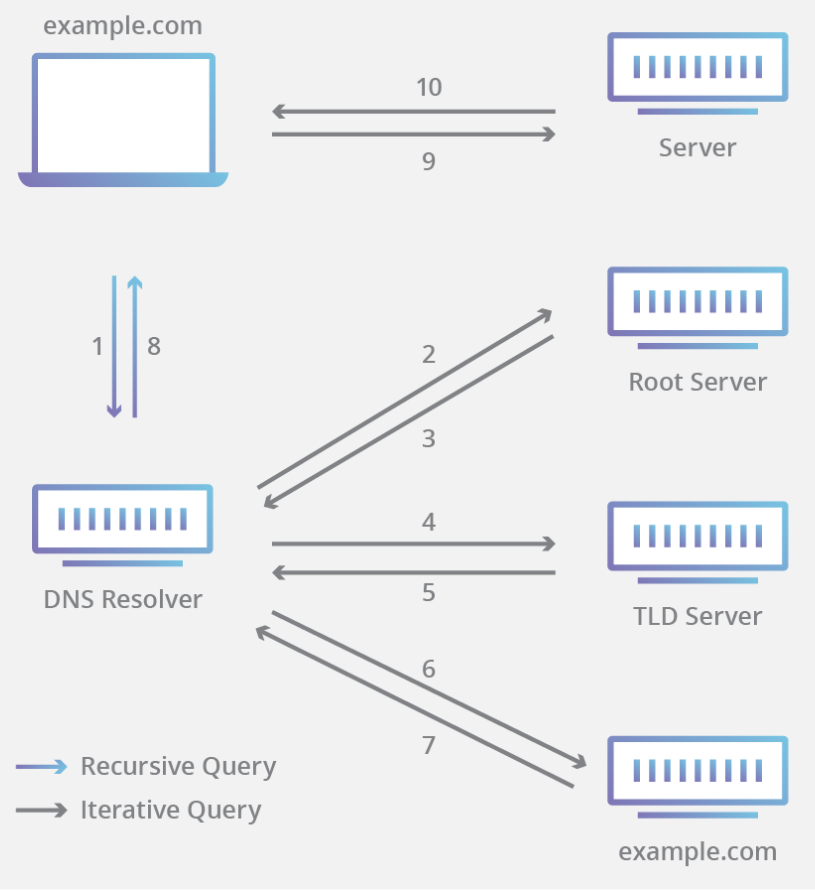
\includegraphics[width=0.25\textwidth]{dns_diagram.png}
\end{figure}

\subsection*{Description du diagramme}
\begin{itemize}
    \item \textbf{Requête récursive} :
    \begin{enumerate}
        \item La requête part de l'ordinateur vers le résolveur DNS.
        \item Le résolveur DNS envoie une requête au serveur racine.
        \item Le serveur racine répond avec les serveurs TLD.
        \item Le résolveur DNS envoie une requête au serveur TLD.
        \item Le serveur TLD répond avec les serveurs autoritaires.
        \item Le résolveur DNS envoie une requête au serveur autoritaire.
        \item Le serveur autoritaire répond avec l'adresse IP de la ressource.
    \end{enumerate}
    \item \textbf{Requête itérative} :
    \begin{enumerate}
        \setcounter{enumi}{7}
        \item Le résolveur DNS renvoie l'adresse IP à l'ordinateur.
        \item L'ordinateur envoie une requête à l'adresse IP du serveur.
        \item Le serveur répond avec la page Web demandée.
    \end{enumerate}
\end{itemize}



\section{HTTP ou Hyper Text Transfer Protocol}

$\blacktriangleright$ Protocole stateless ou \textbf{sans} état, contrairement à \textbf{FTP} ou \textbf{POP} \\

$\blacktriangleright$ Un \textbf{client}, p. ex: navigateur, envoie une requête HTTP à un serveur qui retourne une réponse \\
  
$\blacktriangleright$ La connexion est ensuite rompue, ce qui est simple mais moins efficace \\ 

$\blacktriangleright$ Plusieurs proxy peuvent intervenir entre un client et un serveur \\

$\blacktriangleright$ Chaque acteur peut \textbf{mémoriser} des réponses


\begin{Concept}{Méthode HTTP populaires}{}
\textbf{Syntaxe d'une requête HTTP} : 
\begin{verbatim}
METHOD /path HTTP/version
Header name: valeur
Header name: valeur
[request body]
\end{verbatim}

$\rhd$ \texttt{GET} : Demande d’une ressource, pas de corps \\
$\rhd$ \texttt{POST} : Envoi de paramètres dans le corps de la requête, souvent utilisé pour uploader \\
$\rhd$ \texttt{HEAD} : Seules les en-têtes sont retournées   
\end{Concept}



\begin{EExample}{Commandes HTTP avec \texttt{curl}  }{}
\begin{lstlisting}
(*@\texttt{\textcolor{myb}{// Effectue une requête HTTP/GET}}@*)
% curl https://www.google.ca/
\end{lstlisting}

\begin{lstlisting}
(*@\texttt{\textcolor{myb}{// Affiche les en-têtes de la requête et de la réponse}}@*)
% curl -v https://www.google.ca/
\end{lstlisting}


\begin{lstlisting}
(*@\texttt{\textcolor{myb}{// Réponse indiquant une redirection 301 (Moved Permanently)}}@*)
% curl -v www.iro.umontreal.ca

(*@\texttt{\textcolor{myb}{// Réponse indiquant une redirection 301 vers HTTPS}}@*)
% curl -v http://diro.umontreal.ca

(*@\texttt{\textcolor{myb}{// Réponse indiquant une redirection 307 (Temporary Redirect)}}@*)
% curl -v https://diro.umontreal.ca
\end{lstlisting}


\begin{lstlisting}
(*@\texttt{\textcolor{myb}{// Sauvegarde la sortie dans un fichier nommé} \texttt{out}}@*)
% curl -o out -v \ 
https://diro.umontreal.ca/accueil/

(*@\texttt{\textcolor{myb}{// Affiche contenu du fichier out }}@*)
% cat out
\end{lstlisting}

\end{EExample}


\section{HTTP POST}

\begin{lstlisting}
(*@\texttt{\textcolor{myb}{// Affiche le contenu du fichier} \texttt{x.json}}@*)
% cat x.json
\end{lstlisting}

\begin{lstlisting}
(*@\texttt{\textcolor{myb}{// Envoie une requête POST avec les données de} \texttt{x.json}}@*)
% curl -v -d @x.json https://jsonplaceholder.typicode.com/posts
\end{lstlisting}

\begin{lstlisting}
(*@\texttt{\textcolor{myb}{// Envoie une requête POST avec les données JSON et l'en-tête approprié}}@*)
% curl -v -d @x.json https://jsonplaceholder.typicode.com/posts -H 'Content-Type: application/json'
\end{lstlisting}

\begin{lstlisting}
(*@\texttt{\textcolor{myb}{// Envoie une requête POST avec les données JSON spécifiées directement}}@*)
% curl -d '{"title": "foo","body": "bar","userId": 1}' https://jsonplaceholder.typicode.com/posts -H 'Content-Type: application/json'
\end{lstlisting}

\section*{HTTP PUT}

\begin{EExample}{Envoyer une requête PUT}{}
\begin{lstlisting}
(*@\texttt{\textcolor{myb}{// Envoie une requête PUT pour mettre à jour la ressource avec l'ID 1}}@*)
% curl -X PUT -v -d '{"id": 101, "title": "foo", "body": "bar", "userId": 1}' https://jsonplaceholder.typicode.com/posts/1 -H 'Content-Type: application/json'
\end{lstlisting}
\end{EExample}


\section{Hôtes virtuels}

\begin{Definitionx}{Hôtes virtuels}{}
Combinaison de DNS et d'en-tête HTTP permettant d'héberger plusieurs sites Web sur une seule adresse IP   
\end{Definitionx}


\begin{EExample}{Exemple de requête \texttt{HTTP}  }{}
 \begin{lstlisting}
(*@\texttt{\textcolor{myb}{// Requête GET envoyée à www.google.ca}}@*)
GET / HTTP/1.1
Host: www.google.ca
User-Agent: curl/7.58.0
Accept: */*

(*@\texttt{\textcolor{myb}{//  sites utilisant des hôtes virtuels}}@*)
http://www.gyoukou.ca/linux1
\end{lstlisting}   
\end{EExample}

\end{multicols*}
    \footnotesize



\begin{multicols*}{2}
\chapter{HTML}

\section{Éléments de syntaxe (XHTML)}
\begin{lstlisting}[style=HTMLDraculaDark]
<!-- Déclaration XML -->
<?xml version="1.0" encoding="iso-8859-1"?>
<!-- Déclaration DOCTYPE -->
<!DOCTYPE html PUBLIC "-//W3C//DTD XHTML 1.0 Transitional//EN"
                      "DTD/xhtml1-transitional.dtd">
<!-- Element racine avec namespace -->
<html xmlns="http://www.w3.org/1999/xhtml">
  <!-- En-tête du document -->
  <head>
    <!-- Titre de la page -->
    <title>Hello World</title>
  </head>
  <!-- Corps du document -->
  <body>
    <!-- Paragraphe de texte -->
    <p>My first Web page.</p>
  </body>
</html>
\end{lstlisting}

\begin{note}{}{}
Les namespaces sont essentiels pour éviter les \textbf{conflits}  de noms et garantir que 
les éléments et attributs sont interprétés correctement par les parseurs et les applications.   
L'\textbf{attribut} \texttt{\textcolor{htmltag}{xmlns}} indique que la balise qui le contient est un namespace.     
\end{note}

\section{Avec validation (XHTML)}

\begin{lstlisting}[style=HTMLDraculaDark]
<!-- Déclaration XML -->
<?xml version="1.0" encoding="utf-8"?>
<!-- Déclaration DOCTYPE stricte -->
<!DOCTYPE html PUBLIC "-//W3C//DTD XHTML 1.0 Strict//EN"
                      "http://www.w3.org/TR/xhtml1/DTD/xhtml1-strict.dtd">
<!-- Element racine avec namespace -->
<html xmlns="http://www.w3.org/1999/xhtml">
  <!-- En-tête du document -->
  <head>
    <!-- Métadonnées, encodage du document -->
    <meta http-equiv="Content-Type" content="text/html; charset=utf-8" />
    <!-- Titre de la page -->
    <title>Bonjour le monde</title>
  </head>
  <!-- Corps du document -->
  <body>
    <!-- Paragraphe de texte -->
    <p>Bonjour le monde.</p>
    <!-- Paragraphe avec style centré -->
    <p style="text-align: center">
      <!-- Lien vers un validateur XHTML avec une image -->
      <a href="http://validator.w3.org/check/referer" title="Valid XHTML 1.0">
        <img src="http://www.iro.umontreal.ca/~felipe/Images/button-xhtml.png"
             width="80" height="15" alt="Valid XHTML 1.0" />
      </a>
    </p>
  </body>
</html>
\end{lstlisting}

\begin{note}{}{}
La spécification d'un \textbf{DOCTYPE} dans un document HTML ou XHTML indique 
au navigateur et aux validateurs de quel type de document il s'agit et quelles règles de syntaxe 
doivent être suivies   
\end{note}
$\blacktriangleright$ \texttt{<!DOCTYPE html PUBLIC} : Indique qu'il s'agit d'un document HTML public.

\vspace{0.5cm}

$\blacktriangleright$ \texttt{"-//W3C//DTD XHTML 1.0 Strict//EN"} : Spécifie que le document suit le DTD (\textbf{Document Type Definition}) \texttt{XHTML 1.0 Strict} et que le \textbf{langage} est l'anglais.

\vspace{0.5cm}

$\blacktriangleright$ \texttt{"http://www.w3.org/TR/xhtml1/DTD/xhtml1-strict.dtd"} : L'URL où la DTD peut être trouvée.



\section{HTML 5}

\begin{lstlisting}[style=HTMLDraculaDark]
<!-- Déclaration DOCTYPE HTML5 -->
<!DOCTYPE html>
<!-- Element racine avec langue -->
<html lang="fr">
  <!-- En-tête du document -->
  <head>
    <!-- Titre de la page -->
    <title>Bonjour le Monde</title>
    <!-- Métadonnées, encodage du document -->
    <meta charset="UTF-8">
  </head>
  <!-- Corps du document -->
  <body>
    Bonjour le monde !
    <!-- Section avec liens et images -->
    <div>
      <a href="http://validator.w3.org/check?uri=referer">
        <img src="../images/html5.png" alt="HTML5 valid !" width=22 />
      </a>
      <a href="http://jigsaw.w3.org/css-validator/check/referer">
        <img src="../images/css3.png" alt="CSS valid !" width=20 />
      </a>
    </div>
  </body>
</html>
\end{lstlisting}

\section{Simplifications de HTML5}

\begin{lstlisting}[style=HTMLDraculaDark]
<!-- Attributs sans guillemets -->
<meta charset=utf-8>
<!-- Attribut avec double guillemets : préférable -->
<meta charset="utf-8">
<!-- Attribut avec guillemet unique : aussi toléré-->
<meta charset='utf-8'>

<!-- Balises auto-fermantes -->
<img src="mon_image" alt="une image" />
<img src="mon_image" alt="une image" >

<!-- Casse des tags non sensible -->
<iMg sRC="mon_image" Alt="une image" >

<!-- Balises html, head et body optionnelles mais fortement recommandées-->
<!doctype html>
<meta charset="utf-8">
<title>Bonjour</title>
<p>bla</p>

<!-- Attributs booléens sans valeur explicite -->
<input type="text" autofocus />
<video autoplay loop controls />
\end{lstlisting}

\begin{note}{}{}
Certains \textbf{navigateurs} sont mieux adapté au standard \texttt{HTML5} que d'autres et certaines 
\textbf{balises} sont mieux supportées sur \texttt{HTML5} que d'autres.     
\end{note}
        \footnotesize

\section{Attributs booléens}
\begin{Definitionx}{Attributs booléens}{}
Un attribut booléen en HTML est un type d'attribut dont la présence indique 
une valeur vraie (\textit{true}) et l'absence indique une valeur fausse 
(\textit{false}). Il n'est pas nécessaire de spécifier une valeur explicite 
comme \texttt{"true"} pour ces attributs, car leur simple présence suffit à 
activer leur fonctionnalité.   
\end{Definitionx}

\begin{lstlisting}[style=HTMLDraculaDark]
<!-- Indiquer qu'une option est sélectionnée. -->
<input type="checkbox" checked>

<!-- Indiquer qu'un élément de formulaire est désactivé. -->
<input type="text" disabled>

<!-- Indiquer qu'un champ de formulaire est en lecture seule -->
<input type="text" readonly>

<!-- Indiquer qu'un champ de formulaire est requis -->
<input type="text" required>
\end{lstlisting}



\section{Inline versus Bloc}

$\blacktriangleright$ \textbf{Éléments inline} : s'affichent dans le flux sans rupture 
(pas de retour chariot) à contrario des éléments \textbf{bloc}.

$\blacktriangleright$ \textbf{Propriété visuelle} : on peut changer la propriété visuelle 
des blocs mais par leur modèle de contenu avec \texttt{display:inline} et \texttt{display:block}.

$\blacktriangleright$ \textbf{Règle} : les éléments en ligne ne peuvent contenir que des 
éléments en ligne.

\begin{lstlisting}[style=HTMLDraculaDark]
<!-- Exemple inline -->
<span>Ceci est un élément inline</span>

<!-- Exemple bloc -->
<div>Ceci est un élément bloc</div>
\end{lstlisting}

$\blacktriangleright$ \textbf{HTML5} : cette distinction n’est pas maintenue en HTML5 au 
profit des catégories de contenu.



\section{Attributs Communs}

$\blacktriangleright$ \textbf{class} : ajoute une propriété afin de scripter les éléments 
ayant cette propriété.
\begin{lstlisting}[style=HTMLDraculaDark]
<!-- Ajouter une classe pour styliser les éléments -->
<h2 class="city">London</h2>
<h2 class="city asian-city">Tokyo</h2>
\end{lstlisting}

$\blacktriangleright$ \textbf{id} : un identificateur unique (dans la page).
\begin{lstlisting}[style=HTMLDraculaDark]
<!-- Ajouter un identifiant unique pour un élément -->
<h1 id="myHeader">My Cities</h1>
\end{lstlisting}

$\blacktriangleright$ \textbf{style} : pour définir des propriétés visuelles de l’élément.
\begin{lstlisting}[style=HTMLDraculaDark]
<!-- Définir le style directement dans l'élément -->
<body style="background-color:powderblue;">
  <h1>This is a heading</h1>
</body>
\end{lstlisting}

$\blacktriangleright$ \textbf{name} : réservé à quelques éléments.
\begin{lstlisting}[style=HTMLDraculaDark]
<!-- Ajouter un nom pour certains éléments -->
<input type="text" name="fullname">
\end{lstlisting}



\section{Retraits et sémantique}
 Certaines balises HTML ont été retirées car leur fonctionnalité peut être mieux gérée par CSS, ce qui sépare 
 le \textbf{style} du \textbf{contenu} et améliore l'accessibilité et la maintenabilité du code.


\begin{note}{}{}
    Les balise \texttt{<b>}, \texttt{<i>}, \texttt{small}, \texttt{cite}, et plusieurs autres 
    du même type sont maintenues 
    en HTML5. Elle ont une sématique non-ambigues
\end{note}
\begin{lstlisting}[style=HTMLDraculaDark]
<!-- Indique une partie de texte ressort visuellement -->
<b>Texte en gras</b>

<!-- Passe de forte emphase à forte importance -->
<strong>Texte important</strong>

<!-- Mots étrangers, techniques, ou citations -->
<i>Texte en italique</i>

<!-- Indiquer les petites lignes -->
<small>Texte en petit</small>

<!-- Ne doit pas baliser un auteur mais les oeuvres -->
<cite>Nom de l'oeuvre</cite>
\end{lstlisting}




\section{Balises structurantes}

\begin{lstlisting}[style=HTMLDraculaDark]
<!-- Section de l'en-tête -->
<header>
  <h1>Titre principal</h1>
</header>

<!-- Section du pied de page -->
<footer>
  <p>&copy; 2024 Mon Site Web</p>
</footer>

<!-- Navigation principale -->
<nav>
  <a href="#accueil">Accueil</a>
  <a href="#contact">Contact</a>
</nav>

<!-- Contenu non essentiel -->
<aside>
  <h2>Publicité</h2>
</aside>

<!-- Article indépendant -->
<article>
  <h2>Mon article</h2>
  <p>Contenu de l'article</p>
</article>

<!-- Section thématique -->
<section>
  <h2>Ma section</h2>
  <p>Contenu de la section</p>
</section>
\end{lstlisting}

$\blacktriangleright$ \textbf{Heure et date} :
\begin{lstlisting}[style=HTMLDraculaDark]
<!-- Date et heure -->
<time datetime="2020-01-14">14 Janvier 2020</time>
<time datetime="2020-01-14T11:30">11h30, le 14 Janvier 2020</time>
\end{lstlisting}

$\blacktriangleright$ \textbf{Figures} :
\begin{lstlisting}[style=HTMLDraculaDark]
<!-- Figure avec légende -->
<figure>
  <img src="image.jpg" alt="Description de l'image">
  <figcaption>Figure 1.2 - Description</figcaption>
</figure>
\end{lstlisting}


\section{Plan de Page}
Concevoir un plan de page c'est \textbf{choisir les bonne balises} pour structurer 
sémantiquement le contenu et ainsi présenter l'information de façon organisée. 

\begin{lstlisting}[style=HTMLDraculaDark]
<!-- Exemple de plan de page -->
<body>
  <article>Ceci est mon article</article>
  <nav>mon fil d'ariane</nav>
  <aside>ma publicité</aside>
  <section>ceci est ma section</section>
</body>

<!-- Plan de page avec titres -->
<body>
  <h1>le titre de body</h1>
  <article>
    <h2>Titre de mon article</h2>
    Ceci est mon article
  </article>
  <nav>
    <h2>navigation</h2>
    mon fil d'ariane
  </nav>
  <aside>
    <h2>aside title</h2>
    ma publicité
  </aside>
  <section>
    <h2>titre de section</h2>
    ceci est ma section
  </section>
</body>
\end{lstlisting}


\section{Canvas}



\begin{lstlisting}[style=HTMLDraculaDark]
<!-- Un élément canvas pour dessiner -->
<canvas id="myCanvas"
        width="400" height="300"
        style="border:1px solid #000000;">
  Pas d'élément canvas
</canvas>

<br />

<!-- Une barre de progression -->
<progress id="progress" max=10000 value="1"></progress>
\end{lstlisting}

\begin{note}{}{}
   Il n'est pas très élégant de mettre du CSS dans le HTML.   
\end{note}



\begin{itemize}
    \item \textbf{Script} : Exemple de script pour manipuler le canvas en JavaScript.
\end{itemize}

\begin{lstlisting}[style=HTMLDraculaDark]
<!-- Obtenir le contexte du canvas -->
var c = document.getElementById("myCanvas");
var ctx = c.getContext("2d");

<!-- Commencer un chemin -->
ctx.beginPath();

<!-- Dessiner un arc -->
ctx.arc(10, 100, 2, 0, 2 * Math.PI);

<!-- Fermer le chemin -->
ctx.closePath();

<!-- Tracer le chemin -->
ctx.stroke();
\end{lstlisting}


\section{Tableaux}


\begin{lstlisting}[style=HTMLDraculaDark]
<!-- Déclaration d'un paragraphe de résumé -->
<p id="summary">
  In the following table, characteristics are given in the second column,
  with the negative side in the left column and the positive side in the right column.
</p>

<!-- Déclaration du tableau -->
<table aria-describedby="summary">
  <caption>Characteristics with positive and negative sides</caption>
  <thead>
    <tr>
      <th id="n">Negative</th>
      <th>Characteristic</th>
      <th>Positive</th>
    </tr>
  </thead>
  <tbody>
    <tr>
      <td headers="n r1">Sad</td>
      <th id="r1">Mood</th>
      <td>Happy</td>
    </tr>
    <tr>
      <td headers="n r2">Failing</td>
      <th id="r2">Grade</th>
      <td>Passing</td>
    </tr>
  </tbody>
</table>
\end{lstlisting}


\begin{note}{}{}
     Noter l’absence de balises fermantes pour les éléments \texttt{th}.   
\end{note}


\begin{lstlisting}[style=HTMLDraculaDark]
<!-- Déclaration d'un tableau avec bordure -->
<table border="1">
  <caption>School auction sign-up sheet</caption>
  <thead>
    <tr>
      <th><label for="e1">Sellers Name</label></th>
      <th><label for="e2">Product for sale</label></th>
      <th><label for="e3">Picture of product</label></th>
      <th><label for="e4">Reserve Price</label></th>
    </tr>
  </thead>
  <tbody>
    <tr>
      <td>Ms Danus</td>
      <td>Doughnuts</td>
      <td>
        <img src="https://example.com/mydoughnuts.png"
             alt="Doughnuts from Ms Danus">
      </td>
      <td>$45</td>
    </tr>
    <tr>
      <td><input id="e1" type="text" name="who" required form="f"></td>
      <td><input id="e2" type="text" name="what" required form="f"></td>
      <td><input id="e3" type="url" name="pic" form="f"></td>
      <td><input id="e4" type="number" step="0.01" min="0" value="0" required form="f"></td>
    </tr>
  </tbody>
</table>
\end{lstlisting}
\section{Syntaxe}

\begin{itemize}
    \item Encapsulation correcte des éléments de formulaire.
\end{itemize}

\begin{lstlisting}[style=HTMLDraculaDark]
<!-- Correctement encapsulé -->
<p><label>Delivery instructions: <textarea name="comments"></textarea></label></p>

<!-- Mauvaise encapsulation -->
<p><label>Delivery instructions:</label> <textarea name="comments"></textarea></p>
\end{lstlisting}

\begin{itemize}
    \item Syntaxe alternative en utilisant des tables pour les étiquettes.
\end{itemize}

\begin{lstlisting}[style=HTMLDraculaDark]
<!-- Syntaxe alternative utilisant des tables -->
<form>
  <table>
    <caption>Example, <label>'s for attribute</caption>
    <tr>
      <th><label for="name">Customer name:</label></th>
      <td><input name="name" id="name"></td>
    </tr>
  </table>
</form>
\end{lstlisting}

\section{Vérification côté client (formulaires)}

\begin{itemize}
    \item \textbf{\texttt{required}}: Rend un champ obligatoire.
\end{itemize}

\begin{lstlisting}[style=HTMLDraculaDark]
<!-- Champ requis -->
<p><label>Customer name: <input name="custname" required></label></p>
\end{lstlisting}

\begin{itemize}
    \item \textbf{\texttt{maxlength}}: Limite le nombre de caractères dans le champ input.
    \item \textbf{\texttt{minlength}}: Définit un nombre minimum de caractères requis.
    \item \textbf{\texttt{pattern}}: Importe des contraintes lors de la validation avec une expression régulière.
\end{itemize}

\begin{lstlisting}[style=HTMLDraculaDark]
<!-- Exemple d'utilisation de pattern -->
<input type="text" pattern="\d{5,6}(?:[-\s]\d{4})?">
\end{lstlisting}


\section{Aider l'utilisateur et le client (formulaire)}

\begin{itemize}
    \item Utilisez \textbf{autocomplete} et \textbf{placeholder} pour faciliter la saisie des informations.
\end{itemize}

\begin{lstlisting}[style=HTMLDraculaDark]
<!-- Exemple d'utilisation de autocomplete et placeholder -->
<label for="frmNameA">Name</label>
<input type="text" name="name" id="frmNameA" placeholder="Full name" required autocomplete="name">

<label for="frmEmailA">Email</label>
<input type="email" name="email" id="frmEmailA" placeholder="name@example.com" required autocomplete="email">

<label for="frmEmailC">Confirm Email</label>
<input type="email" name="emailC" id="frmEmailC" placeholder="name@example.com" required autocomplete="email">

<label for="frmPhoneNumA">Phone</label>
<input type="tel" name="phone" id="frmPhoneNumA" placeholder="+1-555-555-1212" required autocomplete="tel">
\end{lstlisting}


\section{En vrac}

\begin{itemize}
    \item \textbf{\texttt{datalist}}: Permet de fournir des suggestions pour les champs input.
\end{itemize}

\begin{lstlisting}[style=HTMLDraculaDark]
<!-- Exemple d'utilisation de datalist -->
<label for="frmFavChocolate">Favorite Type of Chocolate</label>
<input type="text" name="fav-choc" id="frmFavChocolate" list="chocType">
<datalist id="chocType">
  <option value="white">
  <option value="milk">
  <option value="dark">
</datalist>
\end{lstlisting}

\begin{itemize}
    \item \textbf{\texttt{autofocus}}: Mettre le focus sur un élément input lors du chargement de la page.
\end{itemize}

\begin{lstlisting}[style=HTMLDraculaDark]
<!-- Exemple d'utilisation de autofocus -->
<input type="search" name="search" autofocus>
\end{lstlisting}

\begin{itemize}
    \item Mentionner un input en dehors de l'élément form avec l'attribut \texttt{form}.
\end{itemize}

\begin{lstlisting}[style=HTMLDraculaDark]
<!-- Exemple d'utilisation de l'attribut form -->
<form id="maforme">
  <input type="submit">
</form>
<input type="text" name="mytext" form="maforme">
\end{lstlisting}




\end{multicols*}
\section{Formulaires}
\begin{lstlisting}[style=HTMLDraculaDark]
<!-- Début du formulaire -->
<form method="post" enctype="application/x-www-form-urlencoded" action="https://pizza.example.com/order.cgi">

  <!-- Nom du client -->
  <p><label>Customer name: <input name="custname"></label></p>
  
  <!-- Téléphone -->
  <p><label>Telephone: <input type="tel" name="custtel"></label></p>
  
  <!-- Adresse email -->
  <p><label>E-mail address: <input type="email" name="custemail"></label></p>

  <!-- Taille de la pizza -->
  <fieldset>
    <legend>Pizza Size</legend>
    <p><label><input type="radio" name="size" value="small"> Small</label></p>
    <p><label><input type="radio" name="size" value="medium"> Medium</label></p>
    <p><label><input type="radio" name="size" value="large"> Large</label></p>
  </fieldset>

  <!-- Garnitures de la pizza -->
  <fieldset>
    <legend>Pizza Toppings</legend>
    <p><label><input type="checkbox" name="topping" value="bacon"> Bacon</label></p>
    <p><label><input type="checkbox" name="topping" value="cheese"> Extra Cheese</label></p>
    <p><label><input type="checkbox" name="topping" value="onion"> Onion</label></p>
    <p><label><input type="checkbox" name="topping" value="mushroom"> Mushroom</label></p>
  </fieldset>

  <!-- Heure de livraison préférée -->
  <p><label>Preferred delivery time: <input type="time" min="11:00" max="21:00" step="900" name="delivery"></label></p>
  
  <!-- Instructions de livraison -->
  <p><label>Delivery instructions: <textarea name="comments"></textarea></label></p>
  
  <!-- Bouton de soumission -->
  <p><button type="submit">Submit order</button></p>
  
</form>
\end{lstlisting}


\section{Cools inputs}

\begin{itemize}
    \item En HTML5, il existe de nouveaux types d'input natifs: \textbf{password}, \textbf{color}, \textbf{date}, \textbf{datetime-local}, \textbf{month}, \textbf{week}, \textbf{number}, \textbf{range}.
\end{itemize}

\begin{lstlisting}[style=HTMLDraculaDark]
<!-- Exemple d'utilisation de différents types d'input -->
<p><label>Password: <input type="password" name="pwd" placeholder="12345" required></label></p>

<p><label>Color: <input type="color" name="colour" value="#ff0000"></label></p>

<p><label>Date: <input type="date" name="date" placeholder="YYYY-MM-DD" required></label></p>

<p><label>Date & Time: <input type="datetime-local" name="datetime" placeholder="YYYY-MM-DDTHH:MM" required></label></p>

<p><label>Mois: <input type="month" name="month" placeholder="???"></label></p>

<p><label>Semaine: <input type="week" name="week" placeholder="???"></label></p>

<p><label>Nombre: <input type="number" name="nombre" placeholder="123" min="0" max="100"></label></p>

<p><label>Intervalle: <input type="range" name="range" min="1" max="100" required></label></p>
\end{lstlisting}

\begin{note}{}{}
 L'\textbf{apparence} des ces champs et objets peut varier en fonction de l'appareil et du navigateur 
utilisé pour les afficher (p. ex. \textit{desktop} versus mobile).   
\end{note}



\begin{multicols*}{2}
\section{Élément output}
% Cette diapositive explique l'utilisation de l'élément <output> pour afficher des calculs.

\noindent
L'élément \texttt{<output>} est utilisé pour afficher des résultats de calculs directement dans un formulaire. Cet élément peut référencer des inputs via l'attribut \texttt{for} et affiche une valeur par défaut si aucune autre valeur n'est spécifiée.

\begin{lstlisting}[style=HTMLDraculaDark]
<form oninput="x.value=a.valueAsNumber+b.valueAsNumber">
  0 <input type="range" id="a" name="a" value="50" /> 100 +
  <input type="number" id="b" name="b" value="50"/> =
  <output name="x" for="a b">input please!</output>
  <br />
  <input type="reset" />
</form>
\end{lstlisting}


\section{Marquage sémantique}
% Cette diapositive décrit l'utilisation de RDFa et de Microformats pour le marquage sémantique.

RDFa (Resource Description Framework in attributes) permet de semantiquement annoter du contenu directement dans les attributs des balises HTML en utilisant des vocabulaires partagés.

\begin{lstlisting}[style=HTMLDraculaDark]
<div xmlns:dc="http://purl.org/dc/elements/1.1/" about="http://www.example.com/books/wikinomics">
  In his latest book <span property="dc:title">Wikinomics</span>,
  <span property="dc:creator">Don Tapscott</span> explains deep changes in technology.
  The book is due to be published in <span property="dc:date" content="2006-10-01">October 2006</span>.
</div>
\end{lstlisting}

\noindent
Les microformats ajoutent des marqueurs spécifiques directement dans le HTML. Ils ne sont pas une norme officielle mais sont largement utilisés.

\begin{lstlisting}[style=HTMLDraculaDark]
<div class="vcard">
  <p>
    <span class="fn">Jean Bout</span><br />
    <span class="org">Société Exemple</span><br />
    <span class="tel">604-555-1234</span><br />
    <a class="url" href="http://exemple.com">http://exemple.com</a>
  </p>
</div>
\end{lstlisting}


\section{Microdata}
% Cette diapositive explique l'utilisation des microdonnées pour l'annotation sémantique.

\noindent
Les microdonnées (microdata) sont une norme soutenue par WHATWG. Utilisées par les moteurs de recherche et les navigateurs, elles permettent d'annoter les données structurées en utilisant des attributs spécifiques.

\begin{lstlisting}[style=HTMLDraculaDark]
<div itemscope itemtype="http://schema.org/Movie">
  <h1 itemprop="name">Avatar</h1>
  <div itemprop="director" itemscope itemtype="http://schema.org/Person">
    Director: <span itemprop="name">James Cameron</span>
    (born <time itemprop="birthDate" datetime="1954-08-16">August 16, 1954</time>)
  </div>
  <span itemprop="genre">Science fiction</span>
  <a href="../movies/avatar-theatrical-trailer.html" itemprop="trailer">Trailer</a>
</div>
\end{lstlisting}

\noindent
Depuis 2007, Google recommande d'utiliser JSON-LD pour l'annotation sémantique.

\begin{lstlisting}[style=HTMLDraculaDark]
<script type="application/ld+json">
{
  "@context": "http://schema.org",
  "@type": "Movie",
  "name": "Avatar",
  "director": {
    "@type": "Person",
    "name": "James Cameron",
    "birthDate": "1954-08-16"
  },
  "genre": "Science fiction",
  "trailer": "../movies/avatar-theatrical-trailer.html"
}
</script>
\end{lstlisting}



\section{JSON-LD}
% Cette diapositive montre l'utilisation de JSON-LD pour les annotations sémantiques.

\noindent
JSON-LD (JavaScript Object Notation for Linked Data) est un format de sérialisation pour les données liées (linked data). Il permet de structurer les données de manière compréhensible pour les machines.

\begin{lstlisting}[style=HTMLDraculaDark]
<script type="application/ld+json">
{
  "@id": "http://example.com/2016-04-21#main-event",
  "@context": "http://schema.org",
  "@type": "Event",
  "name": "MainEvent",
  "startDate": "2016-04-21T12:00",
  "subEvent": {
    "@id": "http://example.com/2016-04-21#sub-event",
    "@context": "http://schema.org",
    "@type": "Event",
    "name": "SubEvent",
    "startDate": "2016-04-21T12:00",
    "superEvent": {
      "@id": "http://example.com/2016-04-21#main-event"
    }
  }
}
</script>
\end{lstlisting}


\section{Accessibilité}
% Cette diapositive aborde les préoccupations en matière d'accessibilité avec l'utilisation de <del>.

\noindent
L'élément \texttt{<del>} peut ne pas être annoncé par les technologies d'assistance. Pour résoudre ce problème, il est possible d'utiliser les pseudo-éléments CSS \texttt{::before} et \texttt{::after} pour fournir du contexte.

\begin{lstlisting}[style=HTMLDraculaDark]
del::before, del::after {
  clip-path: inset(100%);
  clip: rect(1px, 1px, 1px, 1px);
  height: 1px;
  overflow: hidden;
  position: absolute;
  white-space: nowrap;
  width: 1px;
}
del::before { content: "[deletion start] "; }
del::after { content: " [deletion end]"; }
\end{lstlisting}

\begin{lstlisting}[style=HTMLDraculaDark]
<p><del>This text has been deleted</del>, here is the rest of the paragraph.</p>
<del><p>This paragraph has been deleted.</p></del>
\end{lstlisting}


\section{Compatibilité HTML5}
% Cette diapositive présente la compatibilité HTML5 et des solutions pour les navigateurs anciens.

\noindent
Les nouveaux éléments HTML5 peuvent être injectés dans la DOM pour les navigateurs anciens à l'aide de html5shiv. Ceci est particulièrement utile pour les versions d'Internet Explorer inférieures à IE9.

\begin{lstlisting}[style=HTMLDraculaDark]
<head>
  <title>Bonjour le Monde</title>
  <meta charset="UTF-8">
  <!--[if lt IE 9]>
    <script src="bower_components/html5shiv/dist/html5shiv.js"></script>
  <![endif]-->
</head>
\end{lstlisting}


\chapter{Accessibilité et Aria}
\begin{Concept}{Enjeux d'accessibilité}{}
    Les compagnies ont intérêt à déployer des efforts pour augmenter l'accessibilité, puisqu'une 
    \textbf{portion significative} de la population est affecté d'une invalidité qui 
    peut affecter l'\textbf{expérience utilisateur} lors de la navigation sur une page Web.   
\end{Concept}

$\blacktriangleright$ Généralement, il y a environ $50$ erreur par page Web. 


$\blacktriangleright$ La complexité des pages Web et le nombre d'éléments par page Web augmente avec le temps 


$\blacktriangleright$ Il y a en moyenne plus d'erreur par page lorsque la complexité d'une page augmente. 

$\blacktriangleright$ Certains CMS comme \texttt{Squarespace} et \texttt{Wix} engendrent moins d'erreur que 
la plupart des autres services. 

\section{WAI-ARIA}
\begin{Definitionx}{WAI-ARIA}{}
    \textit{Web Accessibility Initiative Accessible Rich Internet Applications} est un spécification 
    \texttt{W3C} qui définit des attributs améliorant la sémantique et l'accessibilité d'une page.   
\end{Definitionx}

\begin{EExample}{Propriétés de ARIA}{}
    \begin{lstlisting}[style=HTMLDraculaDark]
<!-- Indique ce qu'un élément fait --> 
role = "navigation"

<!-- Indique une propriété d'un élément -->
aria-required=true

<!-- Indique une condition particulière -->
aria-disabl=true
    \end{lstlisting}
\end{EExample}


\begin{note}{}{}
    ARIA est \textbf{particulièrement utile} lorsque la sémantique n'est pas portée par le nom du tag.   
\end{note}


\begin{EExample}{Complémenter la sémantique d'un tag}{}
\begin{lstlisting}[style=HTMLDraculaDark]
<header>
  <!-- Titre principal -->
  <h1>...</h1>
  <nav role="navigation">
    <!-- Liste de liens de navigation -->
    <ul>...</ul>
    <!-- Formulaire de recherche -->
    <form role="search">
      <!-- Champ de recherche -->
      <!-- search form -->
    </form>
  </nav>
</header>

<main>
  <!-- Article principal -->
  <article role="article">...</article>
  <!-- Contenu complémentaire -->
  <aside role="complementary">...</aside>
</main>

<footer>...</footer>

<!-- Champ de recherche avec ARIA -->
<input type="search" name="q" placeholder="Search query" aria-label="Search through site content"
\end{lstlisting}
>\end{EExample}


\begin{lstlisting}[style=HTMLDraculaDark]
<!-- Section avec changement dynamique -->
<section aria-live="assertive" aria-atomic="true">
  <!-- Titre de la section -->
  <h1>Random quote</h1>
  <!-- Citation -->
  <blockquote>
    <p>...</p>
  </blockquote>
</section>
\end{lstlisting}

\begin{itemize}
  \item \textbf{aria-live} : contrôle la manière dont les changements sont annoncés
  \item \textbf{aria-live="off"} : par défaut, ne rien annoncer
  \item \textbf{aria-live="polite"} : annoncer seulement si l'utilisateur ne fait rien
  \item \textbf{aria-live="assertive"} : annoncer dès que possible
  \item \textbf{aria-atomic="true"} : indiquer que tout le contenu doit être annoncé (pas juste la partie modifiée)
\end{itemize}

Avec en JavaScript
\begin{lstlisting}[style=HTMLDraculaDark]
window.setInterval(showQuote, 10000);
\end{lstlisting}


\section{Quelque chose ne devrait pas être lu ?}

\begin{lstlisting}[style=HTMLDraculaDark]
<!-- Elément caché pour les lecteurs d'écran -->
<span aria-hidden="true">...</span>
\end{lstlisting}

Voir aussi les bonnes règles d'un codage HTML sémantique.

Développer des sites web accessibles est compliqué (il existe des certifications). De bons outils sont disponibles (ex: \textit{accessibility inspector}).

\chapter{CSS}

\section{Jargon} 
\begin{EExample}{Syntaxe}{}
   \begin{lstlisting}[style=HTMLDraculaDark]
<!-- Propriété : nom spécifique représentant un aspect --> 
font-weight 

<!-- Sélecteur : désigne des éléments du DOM --> 
p ul 

<!-- Règle : selecteur: valeur --> 
color:red
   \end{lstlisting} 
\end{EExample}

\paragraph{3 Types de CSS}{}
Il y a trois types de CSS
\begin{lstlisting}[style=HTMLDraculaDark]
<!-- Inline --> 
<h1 style="color: red;"> Chapter 1. </h1>

<!-- Style interne -->
    <head>
        <style>
            body {background-color: powderblue;}
            h1 {color: blue;}
            p {color: red;}
        </style>
</head>

<!-- Style externe -->  
<head>
    <link href="path/to/file.css" rel="stylesheet" type="text/css">
</head>
\end{lstlisting}
\section{Sélecteurs}
\paragraph{Sélecteurs de base} Ici

\begin{lstlisting}[style=CSSDraculaLight]
/* Sélecteur universel */
/* Sélectionne tous les éléments */
* {
  /* règles de style ici */
}

/* Sélecteur de type */
/* Sélectionne tous les éléments du nom donné */
input {
  /* règles de style pour les éléments <input> */
}

/* Sélecteur de classe */
/* Sélectionne tous les éléments avec la classe donnée */
.index {
  /* règles de style pour les éléments avec classe "index" */
}

/* Sélecteur d'ID */
/* Sélectionne un élément basé sur la valeur de son attribut id */
#toc {
  /* règles de style pour l'élément avec ID "toc" */
}

/* Sélecteur d'attribut */
/* Sélectionne tous les éléments qui ont l'attribut donné */
[autoplay] {
  /* règles de style pour les éléments avec l'attribut autoplay */
}

/* Sélecteur d'attribut avec valeur spécifique */
/* Sélectionne les éléments avec un attribut égal à une certaine valeur */
[attr=value] {
  /* règles de style ici */
}

/* Sélecteur d'attribut avec valeur contenant un mot spécifique */
/* Sélectionne les éléments avec un attribut contenant un mot spécifique */
[attr~=value] {
  /* règles de style ici */
}

/* Sélecteur d'attribut avec valeur commençant par une chaîne spécifique */
/* Sélectionne les éléments avec un attribut commençant par une chaîne spécifique */
[attr^=value] {
  /* règles de style ici */
}

/* Sélecteur d'attribut avec valeur se terminant par une chaîne spécifique */
/* Sélectionne les éléments avec un attribut se terminant par une chaîne spécifique */
[attr$=value] {
  /* règles de style ici */
}
\end{lstlisting}



\paragraph{Sélecteurs d'attributs} Ici

\begin{lstlisting}[style=CSSDraculaLight]
/* Sélectionne un élément avec l'attribut att */
[att] { color: red; }
/* Sélectionne un élément avec l'attribut att ayant la valeur val */
[att=val] { color: green; }
/* Sélectionne un élément avec l'attribut att ayant la valeur val */
[att~=val] { color: blue; }
/* Sélectionne un élément avec l'attribut att dont la valeur commence par val */
[att^=val] { color: purple; }
/* Sélectionne un élément avec l'attribut att dont la valeur se termine par val */
[att$=val] { color: orange; }
/* Sélectionne un élément avec l'attribut att contenant val */
[att*=val] { color: pink; }
\end{lstlisting}

\paragraph{Selecteur de de groupes} Ici

\begin{lstlisting}[style=CSSDraculaLight]
/* Sélectionne les éléments span et div */
div, span { font-family: sans-serif; }
/* Exemple avec erreur */
h1, h2..foo, h3 { font-family: sans-serif; }
\end{lstlisting}

\section{Combinateurs}
\paragraph{Combinateur} Ici
\begin{lstlisting}[style=CSSDraculaLight]
/* Combinateur de descendant : sélectionne les éléments qui sont des descendants d'un autre élément */
A B { color: blue; }
/* Sélectionne tous les éléments <span> qui sont à l'intérieur d'un élément <div> */
div span { color: red; }

/* Combinateur de l'enfant : sélectionne les éléments qui sont des enfants directs d'un autre élément */
A > B { color: green; }
/* Sélectionne tous les éléments <li> qui sont des enfants directs d'un élément <ul> */
ul > li { color: yellow; }

/* Combinateur de frères généraux : sélectionne les frères d'un élément */
A ~ B { color: purple; }
/* Sélectionne tous les éléments <span> qui suivent un élément <p>, immédiatement ou non */
p ~ span { color: orange; }

/* Combinateur de frères adjacents : sélectionne les frères adjacents d'un élément */
A + B { color: pink; }
/* Sélectionne tous les éléments <p> qui suivent directement un élément <h2> */
h2 + p { color: brown; }

/* Combinateur de colonne : sélectionne les noeuds qui appartiennent à une colonne */
A || B { color: cyan; }
/* Sélectionne tous les éléments <td> qui appartiennent à la portée de l'élément <col> */
col || td { color: teal; }
\end{lstlisting}

\section{Pseudo-classes}
\paragraph{Pseudo-classes} Ici

\begin{lstlisting}[style=CSSDraculaLight]
/* La pseudo-classe :link s'applique aux liens qui n'ont pas encore été visités */
a:link { color: blue; }

/* La pseudo-classe :visited s'applique une fois que le lien a été visité par l'utilisateur */
a:visited { color: purple; }

/* La pseudo-classe :hover s'applique lorsque l'utilisateur désigne un élément avec un dispositif de pointage */
a:hover { color: green; }

/* La pseudo-classe :active s'applique lorsqu'un élément est activé par l'utilisateur */
a:active { color: red; }

/* La pseudo-classe :focus s'applique lorsqu'un élément a le focus */
input:focus { border-color: yellow; }

/* Autres pseudo-classes */
:checked { background-color: orange; }
:root { font-size: 16px; }
:nth-child(odd) { background-color: #ccc; }
:nth-child(even) { background-color: #fff; }
:first-child { font-weight: bold; }
:last-child { font-weight: light; }
:only-child { font-style: italic; }
:empty { display: none; }
:not(.active) { display: block; }
\end{lstlisting}

\section{Psuedo-éléments}

\paragraph{Pseudo-éléments} Ici

\begin{lstlisting}[style=CSSDraculaLight]
/* Pseudo-éléments : utilisés pour styliser des parties spécifiées d'un élément */
/* Sélectionne la première ligne d'un paragraphe */
p::first-line { text-transform: uppercase; }

/* Sélectionne la première lettre d'un paragraphe */
p::first-letter { color: green; font-size: 200%; }

/* Insère du contenu avant un élément */
p::before { content: "Note : "; color: red; }

/* Insère du contenu après un élément */
p::after { content: " Fin."; color: blue; }
\end{lstlisting}



\section{Fonte}
\paragraph{Fontes CSS} Ici 
 \begin{lstlisting}[style=CSSDraculaLight]
p {
    font-family: "Times New Roman", Times, serif; /* Spécifie les polices de caractères pour les éléments <p> */
    /* "Times New Roman" est la police souhaitée */
    /* Times est la police générique par défaut */
}
\end{lstlisting}



\section{Modèle de boîte}
\paragraph{Modèle de boîte CSS} Ici

\begin{lstlisting}[style=CSSDraculaLight]
/* Modèle de boîte pour les éléments HTML */
body { 
    margin: 2em; /* Tous les marges sont définies à 2em */
}

body { 
    margin: 1em 2em; /* Top & Bottom = 1em, Right & Left = 2em */
}

body { 
    margin: 1em 2em 3em 2em; /* Top=1em, Right=2em, Bottom=3em, Left=2em */
}

/* La règle ci-dessus est équivalente à celle ci-dessous */
body {
    margin-top: 1em;
    margin-right: 2em;
    margin-bottom: 3em;
    margin-left: 2em; /* Copié du coté opposé (droite) */
}
\end{lstlisting}

\section{Unités de mesure}
\paragraph{Unités de mesure en CSS} Ic i

\begin{lstlisting}[style=CSSDraculaLight]
.outer {
    border: 5px solid black; /* Bordure de 5px, couleur noire */
}

.box {
    padding: 10px; /* Espace intérieur de 10px */
    width: calc(90% - 30px); /* Largeur calculée comme 90% moins 30px */
    background-color: rebeccapurple; /* Couleur de fond */
    color: white; /* Couleur du texte */
}

.foo {
    --widthA: 100px; /* Variable CSS pour la largeur */
    --widthB: calc(var(--widthA) / 2); /* Calcul de largeur basé sur une variable */
    --widthC: calc(var(--widthB) / 2); /* Calcul de largeur basé sur une autre variable */
    width: var(--widthC); /* Utilisation de la variable pour définir la largeur */
}
\end{lstlisting}


\section{Box-sizing}
\paragraph{Box-sizing}
La propriété \texttt{box-sizing} permet de contrôler la façon dont la largeur et la hauteur des éléments sont calculées.

\begin{lstlisting}[style=CSSDraculaLight]
/* Par défaut, box-sizing est content-box */
.box1 {
    box-sizing: content-box;
    width: 100px; /* la largeur inclut uniquement le contenu */
    padding: 10px; /* le padding est ajouté à la largeur */
    border: 5px solid black; /* la bordure est ajoutée à la largeur */
}

/* Avec border-box, le padding et la bordure sont inclus dans la largeur */
.box2 {
    box-sizing: border-box;
    width: 100px; /* la largeur inclut le contenu, le padding et la bordure */
    padding: 10px;
    border: 5px solid black;
}
\end{lstlisting}


\paragraph{Flexbox}
Le modèle Flexbox offre une manière simple et puissante d'agencer les éléments dans un conteneur.

\begin{lstlisting}[style=CSSDraculaLight]
/* Conteneur flex */
.container {
    display: flex;
    justify-content: space-between; /* espace entre les éléments */
    align-items: center; /* centrer les éléments verticalement */
}

/* Eléments flex */
.item {
    flex: 1; /* prendre tout l'espace disponible */
    padding: 10px;
    margin: 5px;
    background-color: lightblue;
    border: 1px solid blue;
}
\end{lstlisting}


\section{CSS Reset}
Le concept de CSS reset consiste à normaliser les styles par défaut de tous les navigateurs pour éviter les incohérences de rendu. normalize.css est une des bibliothèques les plus populaires pour cela.


\section*{CSS Grid}

CSS Grid Layout est une méthode puissante pour créer des mises en page en deux dimensions dans le web design. Il permet de définir à la fois des colonnes et des lignes, offrant ainsi une grande flexibilité pour disposer les éléments sur une page.







\paragraph{Conteneur de grille}
Le conteneur de grille est l'élément sur lequel on applique \texttt{display: grid}. C'est le parent direct de tous les éléments de la grille.

\begin{lstlisting}[style=CSSDraculaLight]
.container {
  display: grid;  /* Définir un conteneur de grille */
  grid-template-columns: repeat(3, 1fr);  /* Définir un modèle de colonnes */
  grid-template-rows: auto;  /* Définir un modèle de lignes */
}
\end{lstlisting}

HTML correspondant :
\begin{lstlisting}[style=HTMLDraculaDark]
<!DOCTYPE html>
<html lang="fr">
<head>
    <meta charset="UTF-8">
    <meta name="viewport" content="width=device-width, initial-scale=1.0">
    <title>Conteneur de Grille</title>
    <style>
        .container {
            display: grid;
            grid-template-columns: repeat(3, 1fr);
            grid-template-rows: auto;
        }
    </style>
</head>
<body>
    <div class="container">
        <div class="item">Item 1</div>
        <div class="item">Item 2</div>
        <div class="item">Item 3</div>
        <div class="item">Item 4</div>
        <div class="item">Item 5</div>
        <div class="item">Item 6</div>
    </div>
</body>
</html>
\end{lstlisting}

\paragraph{Définition des lignes et colonnes}
Les lignes et colonnes peuvent être définies explicitement en utilisant \texttt{grid-template-columns} et \texttt{grid-template-rows}.

\begin{lstlisting}[style=CSSDraculaLight]
.container {
  display: grid;
  grid-template-columns: 100px 50px auto;  /* Largeur des colonnes */
  grid-template-rows: 80px auto 80px;  /* Hauteur des lignes */
  column-gap: 10px;  /* Espace entre les colonnes */
  row-gap: 15px;  /* Espace entre les lignes */
}
\end{lstlisting}

HTML correspondant :
\begin{lstlisting}[style=HTMLDraculaDark]
<!DOCTYPE html>
<html lang="fr">
<head>
    <meta charset="UTF-8">
    <meta name="viewport" content="width=device-width, initial-scale=1.0">
    <title>Définition des Lignes et Colonnes</title>
    <style>
        .container {
            display: grid;
            grid-template-columns: 100px 50px auto;
            grid-template-rows: 80px auto 80px;
            column-gap: 10px;
            row-gap: 15px;
        }
    </style>
</head>
<body>
    <div class="container">
        <div class="item">Item 1</div>
        <div class="item">Item 2</div>
        <div class="item">Item 3</div>
        <div class="item">Item 4</div>
        <div class="item">Item 5</div>
        <div class="item">Item 6</div>
        <div class="item">Item 7</div>
        <div class="item">Item 8</div>
        <div class="item">Item 9</div>
    </div>
</body>
</html>
\end{lstlisting}

\paragraph{Positionnement des éléments}
Les éléments peuvent être positionnés dans la grille en utilisant \texttt{grid-column} et \texttt{grid-row}.

\begin{lstlisting}[style=CSSDraculaLight]
.item-a {
  grid-column-start: 2;  /* Commence à la 2e colonne */
  grid-column-end: 4;  /* Se termine à la 4e colonne */
  grid-row-start: 1;  /* Commence à la 1re ligne */
  grid-row-end: 3;  /* Se termine à la 3e ligne */
}
\end{lstlisting}

HTML correspondant :
\begin{lstlisting}[style=HTMLDraculaDark]
<!DOCTYPE html>
<html lang="fr">
<head>
    <meta charset="UTF-8">
    <meta name="viewport" content="width=device-width, initial-scale=1.0">
    <title>Positionnement des Eléments</title>
    <style>
        .container {
            display: grid;
            grid-template-columns: repeat(4, 1fr);
            grid-template-rows: repeat(3, 1fr);
        }
        .item-a {
            grid-column-start: 2;
            grid-column-end: 4;
            grid-row-start: 1;
            grid-row-end: 3;
        }
    </style>
</head>
<body>
    <div class="container">
        <div class="item-a">Item A</div>
        <div class="item">Item 1</div>
        <div class="item">Item 2</div>
        <div class="item">Item 3</div>
        <div class="item">Item 4</div>
        <div class="item">Item 5</div>
        <div class="item">Item 6</div>
        <div class="item">Item 7</div>
        <div class="item">Item 8</div>
    </div>
</body>
</html>
\end{lstlisting}









\paragraph{Définir une grille}
Pour créer une grille de base en CSS, on utilise la propriété `grid-template-columns` pour définir les colonnes. Le code suivant illustre comment définir une grille avec différentes configurations de colonnes.

\begin{lstlisting}[style=CSSDraculaLight]
.container {
  grid-template-columns: repeat(3, 20px); /* Définir une grille avec 3 colonnes de 20px de largeur chacune */
}

.item {
  grid-column-start: col-start 2; /* Positionner un élément pour qu'il commence à la 2ème colonne */
}

.container {
  grid-template-columns: 1fr 1fr 1fr; /* Définir une grille avec 3 colonnes qui se répartissent uniformément la largeur disponible */
}

.container {
  grid-template-columns: 1fr 50px 1fr 1fr; /* Définir une grille avec 4 colonnes, la deuxième colonne ayant une largeur de 50px, les autres colonnes se répartissant uniformément */
}
\end{lstlisting}

HTML correspondant :
\begin{lstlisting}[style=HTMLDraculaDark]
<div class="container">
  <div class="item">Item 1</div>
  <div class="item">Item 2</div>
  <div class="item">Item 3</div>
</div>
\end{lstlisting}

\paragraph{Définir une grille avancée}
Pour créer une grille plus complexe avec des zones nommées, on utilise les propriétés `grid-area` et `grid-template-areas`. Le code suivant montre comment créer une grille avec des zones spécifiques pour l'en-tête, le contenu principal, la barre latérale et le pied de page.

\begin{lstlisting}[style=CSSDraculaLight]
.item-a {
  grid-area: header; /* Définir la zone de la grille pour l'en-tête */
}

.item-b {
  grid-area: main; /* Définir la zone de la grille pour le contenu principal */
}

.item-c {
  grid-area: sidebar; /* Définir la zone de la grille pour la barre latérale */
}

.item-d {
  grid-area: footer; /* Définir la zone de la grille pour le pied de page */
}

.container {
  display: grid;
  grid-template-columns: 50px 50px 50px 50px; /* Définir les colonnes de la grille avec 4 colonnes de 50px */
  grid-template-rows: auto; /* Définir les lignes de la grille avec une hauteur automatique */
  grid-template-areas:
    "header header header header"
    "main main . sidebar"
    "footer footer footer footer"; /* Définir les zones de la grille : une grille 4x3, où '.' indique une cellule vide */
}
\end{lstlisting}

HTML correspondant :
\begin{lstlisting}[style=HTMLDraculaDark]
<div class="container">
  <div class="item-a">Header</div>
  <div class="item-b">Main</div>
  <div class="item-c">Sidebar</div>
  <div class="item-d">Footer</div>
</div>
\end{lstlisting}

\paragraph{Espacement des cellules}
Pour définir l'espacement entre les cellules d'une grille, on utilise les propriétés `column-gap` et `row-gap`. Le code suivant montre comment définir ces espacements pour une grille donnée.

\begin{lstlisting}[style=CSSDraculaLight]
.container {
  grid-template-columns: 100px 50px 100px; /* Définir les colonnes de la grille avec des largeurs spécifiques */
  grid-template-rows: 80px auto 80px; /* Définir les lignes de la grille avec des hauteurs spécifiques */
  column-gap: 10px; /* Définir l'espace entre les colonnes */
  row-gap: 15px; /* Définir l'espace entre les lignes */
}
\end{lstlisting}

HTML correspondant :
\begin{lstlisting}[style=HTMLDraculaDark]
<div class="container">
  <div class="item">Item 1</div>
  <div class="item">Item 2</div>
  <div class="item">Item 3</div>
  <div class="item">Item 4</div>
  <div class="item">Item 5</div>
  <div class="item">Item 6</div>
  <div class="item">Item 7</div>
  <div class="item">Item 8</div>
  <div class="item">Item 9</div>
</div>
\end{lstlisting}

\paragraph{Positionner des items}
Pour positionner des éléments spécifiques dans une grille, on utilise les propriétés `grid-column-start`, `grid-column-end`, `grid-row-start` et `grid-row-end`. Le code suivant montre comment positionner un élément dans une grille et comment utiliser des raccourcis pour simplifier le positionnement.

\begin{lstlisting}[style=CSSDraculaLight]
.item-a {
  grid-column-start: 2; /* Positionner l'élément pour qu'il commence à la 2ème colonne */
  grid-column-end: five; /* Positionner l'élément pour qu'il s'étende jusqu'à la colonne 'five' */
  grid-row-start: row1-start; /* Positionner l'élément pour qu'il commence à la ligne 'row1-start' */
  grid-row-end: 3; /* Positionner l'élément pour qu'il s'étende jusqu'à la 3ème ligne */
}

/* Utilisation des raccourcis pour positionner les éléments */
.item-a {
  grid-column: 2 / span 3; /* Positionner l'élément pour qu'il commence à la 2ème colonne et s'étende sur 3 colonnes */
  grid-row: 1 / 3; /* Positionner l'élément pour qu'il commence à la 1ère ligne et s'étende jusqu'à la 3ème ligne */
}
\end{lstlisting}

HTML correspondant :
\begin{lstlisting}[style=HTMLDraculaDark]
<div class="container">
  <div class="item-a">Item A</div>
  <div class="item-b">Item B</div>
  <div class="item-c">Item C</div>
  <div class="item-d">Item D</div>
  <div class="item-e">Item E</div>
  <div class="item-f">Item F</div>
  <div class="item-g">Item G</div>
  <div class="item-h">Item H</div>
  <div class="item-i">Item I</div>
</div>
\end{lstlisting}

\begin{itemize}
  \item \textbf{Grid Container} : Élément parent avec \texttt{display: grid}.
  \item \textbf{Grid Item} : Enfants directs du conteneur de grille.
  \item \textbf{Grid Line} : Lignes qui divisent la grille en colonnes et rangées.
  \item \textbf{Grid Cell} : Espace entre deux lignes de grille adjacentes.
  \item \textbf{Grid Track} : Espace entre deux lignes de grille.
  \item \textbf{Grid Area} : Espace entouré par quatre lignes de grille.
\end{itemize}





\section{La Cascade CSS}

La cascade est le mécanisme par lequel les styles CSS sont appliqués aux éléments HTML. Les règles de style proviennent de trois sources principales : l'agent utilisateur (navigateur), l'auteur de la page (le plus souvent), et l'utilisateur de la page. Les règles s'appliquant à un élément sont triées par origine et importance, ce qui détermine leur priorité.


\paragraph{Conflit de sélecteurs}

Dans cet exemple, nous avons deux sélecteurs en conflit : un sélecteur ID et un sélecteur de classe. Le sélecteur ID a une spécificité plus élevée et sera donc appliqué.

\begin{lstlisting}[style=CSSDraculaLight]
#someElement p {
  color: blue; /* Ce style sera appliqué car l'ID a une spécificité plus élevée */
}

p.awesome {
  color: red; /* Ce style sera ignoré */
}
\end{lstlisting}

\begin{lstlisting}[style=HTMLDraculaDark]
<div id="someElement">
  <p class="awesome">halo</p>
</div>
\end{lstlisting}

\paragraph{Utilisation de !important}

L'utilisation de \texttt{!important} permet de surcharger les autres déclarations, indépendamment de la spécificité.

\begin{lstlisting}[style=CSSDraculaLight]
p.awesome {
  color: red !important; /* Ce style sera appliqué car il utilise !important */
}
\end{lstlisting}

\begin{lstlisting}[style=HTMLDraculaDark]
<div id="someElement">
  <p class="awesome">halo</p>
</div>
\end{lstlisting}

\paragraph{Conflit de sélecteurs de type}

Dans cet exemple, nous avons un conflit entre deux sélecteurs de type. Les conflits sont gérés par règle indépendamment (ici, \texttt{background-color} et \texttt{color}).

\begin{lstlisting}[style=CSSDraculaLight]
p {
  background-color: yellow; /* Fond jaune pour tous les <p> */
  color: blue; /* Texte bleu pour tous les <p> */
}

p[rel] {
  background-color: greenyellow; /* Fond vert-jaune pour les <p> avec attribut rel */
}
\end{lstlisting}

\begin{lstlisting}[style=HTMLDraculaDark]
<div>
  <p>hallo</p> <!-- Fond jaune, texte bleu -->
  <p rel="woh!">le monde</p> <!-- Fond vert-jaune, texte bleu -->
</div>
\end{lstlisting}

Ces exemples montrent comment les différentes règles CSS sont appliquées en fonction de leur spécificité et de leur ordre dans la cascade. Les exemples HTML fournis montrent comment les styles CSS affectent les éléments HTML correspondants.


\section*{L'ordre compte également}

À spécificité égale, l’ordre compte :
\begin{itemize}
    \item L’ordre dans lequel les fichiers de style sont chargés
    \item L’ordre des règles dans un fichier
\end{itemize}

\begin{verbatim}
Les règles définies plus bas dans un fichier écrasent celles définies plus haut.
\end{verbatim}

\url{https://css-tricks.com/precedence-css-order-css-matters/}

\section*{Héritage}

Certaines propriétés CSS appliquées à un élément vont être héritées par les éléments fils :
\begin{itemize}
    \item Pas toutes les propriétés
        \begin{itemize}
            \item Savoir lesquelles sont héritées requiert bon sens et connaissance de CSS
            \item ex: font-family est héritée, pas les propriétés liées aux marges
        \end{itemize}
    \item Pas en cas de conflit
        \begin{itemize}
            \item Un enfant qui définit une propriété a préséance sur le mécanisme d’héritage
        \end{itemize}
\end{itemize}

Il est possible de contrôler le mécanisme d’héritage :
\begin{itemize}
    \item \texttt{inherit}, \texttt{initial}, \texttt{unset}, \texttt{revert}
\end{itemize}

\begin{lstlisting}[style=CSSDraculaLight]
li {
  margin-left: inherit;  /* La marge gauche des éléments <li> héritent des valeurs du parent */
}
\end{lstlisting}

\begin{lstlisting}[style=HTMLDraculaDark]
<ul>
  <li>Item 1</li>
  <li>Item 2</li>
  <li>Item 3</li>
</ul>
\end{lstlisting}


\section{Les Media Queries en CSS}

\paragraph{Media Queries}
Les media queries permettent d'appliquer des styles CSS différents en fonction du type de média (écran, impression, etc.) ou des caractéristiques de l'appareil (largeur d'écran, résolution, etc.). Elles sont très utiles pour rendre un site web réactif.

\begin{lstlisting}[style=CSSDraculaLight]
@media print {
  body { font-size: 10pt; }  /* Style pour impression */
}

@media screen {
  body { font-size: 13px; }  /* Style pour écran */
}

@media screen, print {
  body { line-height: 1.2; }  /* Style commun pour écran et impression */
}

@media only screen and (min-width: 320px) and (max-width: 480px) and (resolution: 150dpi) {
  body { line-height: 1.4; }  /* Style pour certains écrans seulement */
}
\end{lstlisting}

\begin{lstlisting}[style=HTMLDraculaDark]
<!DOCTYPE html>
<html>
<head>
  <title>Exemple Media Queries</title>
  <link rel="stylesheet" href="style.css">
</head>
<body>
  <p>Ce texte est redimensionné et interligne selon le type de média.</p>
</body>
</html>
\end{lstlisting}

\paragraph{Breakpoints}
Les breakpoints sont des points de rupture où les styles CSS changent en fonction de la taille de l'écran. Ils permettent de créer des mises en page réactives.

\begin{lstlisting}[style=CSSDraculaLight]
// Extra small devices (portrait phones, less than 576px)
@media (min-width: 576px) { ... }  /* Pas de media query pour `xs` */

// Small devices (landscape phones, 576px and up)
@media (min-width: 576px) { ... }  

// Medium devices (tablets, 768px and up)
@media (min-width: 768px) { ... }  

// Large devices (desktops, 992px and up)
@media (min-width: 992px) { ... }  

// Extra large devices (large desktops, 1200px and up)
@media (min-width: 1200px) { ... }  

// On parle souvent de breakpoint.
\end{lstlisting}

\begin{lstlisting}[style=HTMLDraculaDark]
<!DOCTYPE html>
<html>
<head>
  <title>Exemple Breakpoints</title>
  <link rel="stylesheet" href="style.css">
</head>
<body>
  <div class="container">
    <p>Ce contenu s'adapte à la taille de l'écran grâce aux breakpoints.</p>
  </div>
</body>
</html>
\end{lstlisting}






\paragraph{Sass Variables}
Les variables Sass permettent de stocker des valeurs que vous réutiliserez plusieurs fois dans votre feuille de style.

\begin{lstlisting}[style=CSSDraculaLight]
$font-stack:    Helvetica, sans-serif;  /* Définition d'une variable pour la pile de polices */
$primary-color: #333;  /* Définition d'une variable pour la couleur principale */

body {
  font: 100% $font-stack;  /* Utilisation de la variable $font-stack */
  color: $primary-color;   /* Utilisation de la variable $primary-color */
}
\end{lstlisting}

\begin{lstlisting}[style=HTMLDraculaDark]
<body>
  <p>Texte avec styles Sass</p>
</body>
\end{lstlisting}

\paragraph{Sass Imbrication}
Sass permet l'imbrication des sélecteurs CSS pour améliorer la lisibilité et la maintenance du code.

\begin{lstlisting}[style=CSSDraculaLight]
nav {
  ul {
    margin: 0;  /* Suppression de la marge */
    padding: 0;  /* Suppression du padding */
    list-style: none;  /* Suppression des puces de liste */
  }

  li { 
    display: inline-block;  /* Les éléments de liste sont affichés en ligne */
  }

  a {
    display: block;  /* Les liens sont affichés en blocs */
    padding: 6px 12px;  /* Padding interne des liens */
    text-decoration: none;  /* Suppression du soulignement des liens */
  }
}
\end{lstlisting}

\begin{lstlisting}[style=HTMLDraculaDark]
<nav>
  <ul>
    <li><a href="#">Lien 1</a></li>
    <li><a href="#">Lien 2</a></li>
    <li><a href="#">Lien 3</a></li>
  </ul>
</nav>
\end{lstlisting}

\paragraph{Sass Opérateurs}
Sass permet d'utiliser des opérateurs mathématiques pour manipuler les valeurs CSS.

\begin{lstlisting}[style=CSSDraculaLight]
.container { 
  width: 100%;  /* La largeur du conteneur est de 100% */
}

article[role="main"] {
  float: left;  /* L'article principal flotte à gauche */
  width: 600px / 960px * 100%;  /* Largeur calculée par division et multiplication */
}

aside[role="complementary"] {
  float: right;  /* Le contenu complémentaire flotte à droite */
  width: 300px / 960px * 100%;  /* Largeur calculée par division et multiplication */
}
\end{lstlisting}

\begin{lstlisting}[style=HTMLDraculaDark]
<div class="container">
  <article role="main">Contenu principal</article>
  <aside role="complementary">Contenu complémentaire</aside>
</div>
\end{lstlisting}

\paragraph{Sass Modules}
Sass permet de diviser les styles en modules pour une meilleure organisation du code.

\begin{lstlisting}[style=CSSDraculaLight]
// _base.scss
$font-stack:    Helvetica, sans-serif;  /* Définition d'une variable pour la pile de polices */
$primary-color: #333;  /* Définition d'une variable pour la couleur principale */

body {
  font: 100% $font-stack;  /* Utilisation de la variable $font-stack */
  color: $primary-color;   /* Utilisation de la variable $primary-color */
}

// styles.scss
@use 'base';  /* Importation du module base */

.inverse {
  background-color: base.$primary-color;  /* Utilisation de la variable $primary-color du module base */
  color: white;  /* Définition de la couleur du texte en blanc */
}
\end{lstlisting}

\begin{lstlisting}[style=HTMLDraculaDark]
<body>
  <p class="inverse">Texte inversé</p>
</body>
\end{lstlisting}

\paragraph{Sass Mixins}
Les mixins Sass permettent de définir des blocs de styles réutilisables dans votre feuille de style.

\begin{lstlisting}[style=CSSDraculaLight]
@mixin transform($property) {
  -webkit-transform: $property;  /* Préfixe pour Webkit */
      -ms-transform: $property;  /* Préfixe pour IE */
          transform: $property;  /* Propriété standard */
}

.box { 
  @include transform(rotate(30deg));  /* Utilisation de la mixin transform */
}
\end{lstlisting}

\begin{lstlisting}[style=HTMLDraculaDark]
<div class="box">Contenu transformé</div>
\end{lstlisting}


\section*{Sass Héritage}

L'héritage dans Sass permet de réutiliser des styles communs en étendant une règle à d'autres sélecteurs. Cela aide à réduire la duplication de code et à maintenir une structure CSS plus propre.

\begin{lstlisting}[style=CSSDraculaLight]
/* Ce CSS sera imprimé car %message-shared est étendu */
%message-shared {
  border: 1px solid #ccc;  /* Définir une bordure */
  padding: 10px;  /* Ajouter du padding */
  color: #333;  /* Définir la couleur du texte */
}

/* Ce CSS ne sera pas imprimé car %equal-heights n'est jamais étendu */
%equal-heights {
  display: flex;  /* Utiliser flexbox pour le conteneur */
  flex-wrap: wrap;  /* Permettre le retour à la ligne des éléments flex */
}

.message {
  @extend %message-shared;  /* Etendre les styles de %message-shared */
}

.success {
  @extend %message-shared;  /* Etendre les styles de %message-shared */
  border-color: green;  /* Définir une couleur de bordure verte */
}

.error {
  @extend %message-shared;  /* Etendre les styles de %message-shared */
  border-color: red;  /* Définir une couleur de bordure rouge */
}

.warning {
  @extend %message-shared;  /* Etendre les styles de %message-shared */
  border-color: yellow;  /* Définir une couleur de bordure jaune */
}
\end{lstlisting}

Voici le code HTML correspondant qui peut être manipulé par ce CSS:

\begin{lstlisting}[style=HTMLDraculaDark]
<div class="message">Message par défaut</div>
<div class="success">Message de succès</div>
<div class="error">Message d'erreur</div>
<div class="warning">Message d'avertissement</div>
\end{lstlisting}

\section*{Sass Préprocesseur}

Sass est un préprocesseur CSS qui ajoute des fonctionnalités puissantes comme les variables, les mixins, et l'héritage. Vous pouvez compiler votre code Sass en CSS avec des commandes simples dans votre terminal.

\begin{lstlisting}[style=CSSDraculaLight]
/* Commandes pour compiler Sass en CSS */
/* Pour une transformation à la demande */
sass --watch input.scss output.css

/* Transformation lors de changements dans les fichiers */
sass --watch app/sass:public/stylesheets
\end{lstlisting}




\chapter{Bootstrap}
Bootstrap permet de styler vos pages sans souffrir avec CSS, il est orienté vers les applications mobiles et offre un modèle de grille par conventions de nommage. Il propose des composants (comme des carrousels et jumbotron) qui sont stylés en CSS avec un beau rendu par défaut et sont faciles à interfacer avec JavaScript. Bootstrap est téléchargeable sous forme de fichiers .css et .js, ou supporté par BootstrapCDN. Se lier à la version du Content Delivery Network est souvent un bon choix.





\paragraph{Pour commencer}
Pour intégrer Bootstrap dans votre projet, ajoutez le lien CSS dans la section \texttt{<head>} de votre document HTML avant toute autre feuille de style et les scripts JavaScript avant la fermeture de la balise \texttt{</body>}.

\begin{lstlisting}[style=CSSDraculaLight]
<link rel="stylesheet" href="https://stackpath.bootstrapcdn.com/bootstrap/4.4.1/css/bootstrap.min.css" integrity="sha384-Vkoo8x4CGs03+Hhxv8T/Q5PaXtkKtu6ug5T0eNV6gBiFeWPGFN9MuhOf23Q9Ifjh" crossorigin="anonymous">
\end{lstlisting}

\begin{lstlisting}[style=CSSDraculaLight]
<script src="https://code.jquery.com/jquery-3.4.1.slim.min.js" integrity="sha384-J6qa4849blE2+poT4WnyKhv5vZF5srPo0iEjwBvKU7imGFAV0wwjlyYfJoRSJoZn" crossorigin="anonymous"></script>
<script src="https://cdn.jsdelivr.net/npm/popper.js@1.16.0/dist/umd/popper.min.js" integrity="sha384-Q6E9RHvbIyZFJoft+2mJbHaEwldvI9IOY5n3zV9zzTtmI3UksdRXvoxfMoA4M" crossorigin="anonymous"></script>
<script src="https://stackpath.bootstrapcdn.com/bootstrap/4.4.1/js/bootstrap.min.js" integrity="sha384-wfSDF2E50Y2D1uUdj003uMBJnjuUd4Ih7YwaYd1qfkfj0Ud8GCE3l0g8ifwB6" crossorigin="anonymous"></script>
\end{lstlisting}

\paragraph{CSS files}
\begin{table}[H]
    \centering
    \begin{tabular}{|l|l|l|l|l|}
        \hline
        \textbf{CSS files} & \textbf{Layout} & \textbf{Content} & \textbf{Components} & \textbf{Utilities} \\
        \hline
        bootstrap.css & Included & Included & Included & Included \\
        bootstrap.min.css & Included & Included & Included & Included \\
        bootstrap-grid.css & Only grid system & Not included & Not included & Only flex utilities \\
        bootstrap-grid.min.css & Only grid system & Not included & Not included & Only flex utilities \\
        bootstrap-reboot.css & Not included & Only Reboot & Not included & Not included \\
        bootstrap-reboot.min.css & Not included & Only Reboot & Not included & Not included \\
        \hline
    \end{tabular}
    \caption{Options d'inclusion de CSS Bootstrap}
\end{table}

\paragraph{JS files}
\begin{table}[H]
    \centering
    \begin{tabular}{|l|l|l|}
        \hline
        \textbf{JS files} & \textbf{Popper} & \textbf{jQuery} \\
        \hline
        bootstrap.bundle.js & Included & Not included \\
        bootstrap.bundle.min.js & Included & Not included \\
        bootstrap.js & Not included & Not included \\
        bootstrap.min.js & Not included & Not included \\
        \hline
    \end{tabular}
    \caption{Options d'inclusion de JS Bootstrap}
\end{table}

\paragraph{Besoin de JavaScript ?}
Bootstrap utilise JavaScript pour plusieurs composants interactifs, notamment les alertes, les boutons de bascule, les carrousels, les collapsibles, les dropdowns, les modals, les tooltips et les popovers, ainsi que le scrollspy. Certains de ces composants nécessitent également Popper.js.

\paragraph{Breakpoints}
\begin{table}[H]
    \centering
    \begin{tabular}{|l|l|l|}
        \hline
        \textbf{Breakpoint} & \textbf{Class infix} & \textbf{Dimensions} \\
        \hline
        Extra small & None & <576px \\
        Small & sm & $\geq$ 576px \\
        Medium & md & $\geq$ 768px \\
        Large & lg & $\geq$ 992px \\
        Extra large & xl & $\geq$1200px \\
        Extra extra large & xxl & $\geq$ 1400px \\
        \hline
    \end{tabular}
    \caption{Breakpoints Bootstrap}
\end{table}










\section*{Utilisation en CSS}

\begin{lstlisting}[style=CSSDraculaLight]
/* X-Small devices (portrait phones, less than 576px) */
/* No media query for `xs` since this is the default in Bootstrap */

/* Small devices (landscape phones, 576px and up) */
@media (min-width: 576px) {
  /* Styles pour petits appareils */
}

/* Medium devices (tablets, 768px and up) */
@media (min-width: 768px) {
  /* Styles pour appareils moyens */
}

/* Large devices (desktops, 992px and up) */
@media (min-width: 992px) {
  /* Styles pour grands appareils */
}

/* X-Large devices (large desktops, 1200px and up) */
@media (min-width: 1200px) {
  /* Styles pour très grands appareils */
}

/* XX-Large devices (larger desktops, 1400px and up) */
@media (min-width: 1400px) {
  /* Styles pour très très grands appareils */
}
\end{lstlisting}

\begin{lstlisting}[style=HTMLDraculaDark]
<!DOCTYPE html>
<html lang="fr">
<head>
    <meta charset="UTF-8">
    <meta name="viewport" content="width=device-width, initial-scale=1.0">
    <title>Exemple de Media Queries</title>
    <link rel="stylesheet" href="styles.css">
</head>
<body>
    <div class="content">
        <p>Contenu de démonstration pour différentes tailles d'appareil.</p>
    </div>
</body>
</html>
\end{lstlisting}


% Utilisation en SASS
\section*{Utilisation en SASS}

\begin{lstlisting}[style=CSSDraculaLight]
/* Source mixins */

/* No media query necessary for xs breakpoint as it's effectively */
@include media-breakpoint-up(sm) {
  /* Styles pour petits appareils */
}
@include media-breakpoint-up(md) {
  /* Styles pour appareils moyens */
}
@include media-breakpoint-up(lg) {
  /* Styles pour grands appareils */
}
@include media-breakpoint-up(xl) {
  /* Styles pour très grands appareils */
}
@include media-breakpoint-up(xxl) {
  /* Styles pour très très grands appareils */
}

/* Usage */
/* Example: Hide starting at `min-width: 0`, and then show at the `sm` breakpoint */
.custom-class {
  display: none;
}
@include media-breakpoint-up(sm) {
  .custom-class {
    display: block;
  }
}
\end{lstlisting}

\begin{lstlisting}[style=HTMLDraculaDark]
<!DOCTYPE html>
<html lang="fr">
<head>
    <meta charset="UTF-8">
    <meta name="viewport" content="width=device-width, initial-scale=1.0">
    <title>Exemple de SASS Media Queries</title>
    <link rel="stylesheet" href="styles.css">
</head>
<body>
    <div class="custom-class">
        <p>Ce contenu s'affiche sur les petits appareils et plus grands.</p>
    </div>
</body>
</html>
\end{lstlisting}


% Containers
\section*{Containers}

\noindent Il existe trois types de conteneurs en Bootstrap :
\begin{itemize}
    \item \texttt{container} : taille fixe
    \item \texttt{container-fluid} : 100\% du viewport
    \item \texttt{container-lg} : 100\% du viewport jusqu'au breakpoint spécifié
\end{itemize}

\begin{lstlisting}[style=CSSDraculaLight]
.container {
  /* Styles pour conteneur fixe */
}

.container-fluid {
  width: 100%;
}

.container-lg {
  max-width: 1140px; /* Exemple pour un conteneur lg */
}
\end{lstlisting}

\begin{lstlisting}[style=HTMLDraculaDark]
<!DOCTYPE html>
<html lang="fr">
<head>
    <meta charset="UTF-8">
    <meta name="viewport" content="width=device-width, initial-scale=1.0">
    <title>Exemple de Conteneurs</title>
    <link rel="stylesheet" href="styles.css">
</head>
<body>
    <div class="container">
        <p>Contenu dans un conteneur fixe.</p>
    </div>
    <div class="container-fluid">
        <p>Contenu dans un conteneur fluide.</p>
    </div>
    <div class="container-lg">
        <p>Contenu dans un conteneur lg.</p>
    </div>
</body>
</html>
\end{lstlisting}


% Grille
\section*{Grille}

\noindent Bootstrap utilise une grille de 12 colonnes et 6 breakpoints. Une rangée (\texttt{row}) encapsule des colonnes (\texttt{col}).

\begin{lstlisting}[style=CSSDraculaLight]
.container {
  display: flex;
  flex-wrap: wrap;
}

.row {
  display: flex;
  flex-wrap: wrap;
}

.col {
  flex: 1;
  padding: 15px;
}
\end{lstlisting}

\begin{lstlisting}[style=HTMLDraculaDark]
<!DOCTYPE html>
<html lang="fr">
<head>
    <meta charset="UTF-8">
    <meta name="viewport" content="width=device-width, initial-scale=1.0">
    <title>Exemple de Grille</title>
    <link rel="stylesheet" href="styles.css">
</head>
<body>
    <div class="container">
        <div class="row">
            <div class="col">1 of 2</div>
            <div class="col">2 of 2</div>
        </div>
        <div class="row">
            <div class="col">1 of 3</div>
            <div class="col">2 of 3</div>
            <div class="col">3 of 3</div>
        </div>
    </div>
</body>
</html>
\end{lstlisting}

% Grille (avancée)
\begin{lstlisting}[style=CSSDraculaLight]
.container {
  margin-top: 1rem;
}

.themed-grid-col {
  padding: 15px;
  background-color: rgba(86, 61, 124, 0.15);
  border: 1px solid rgba(86, 61, 124, 0.2);
}
\end{lstlisting}

\begin{lstlisting}[style=HTMLDraculaDark]
<!DOCTYPE html>
<html lang="fr">
<head>
    <meta charset="UTF-8">
    <meta name="viewport" content="width=device-width, initial-scale=1.0">
    <title>Exemple de Grille Avancée</title>
    <link rel="stylesheet" href="styles.css">
</head>
<body>
    <div class="container mt-1">
        <div class="row">
            <div class="col-3 themed-grid-col rounded">1 of 2</div>
            <div class="col themed-grid-col rounded">2 of 2</div>
        </div>
        <div class="row">
            <div class="col-3 themed-grid-col rounded">1 of 3</div>
            <div class="col-6 themed-grid-col rounded">2 of 3</div>
            <div class="col-3 themed-grid-col rounded">3 of 3</div>
        </div>
    </div>
</body>
</html>
\end{lstlisting}





% Colonnes
\section*{Colonnes}

\begin{lstlisting}[style=CSSDraculaLight]
.container {
  text-align: center; /* Centre le texte à l'intérieur du conteneur */
}

.row {
  display: flex;
  justify-content: space-around; /* Répartit uniformément les colonnes */
}

.col {
  flex: 1; /* Chaque colonne prend une part égale de l'espace disponible */
  padding: 10px;
}

.align-self-start {
  align-self: flex-start; /* Aligne cette colonne en haut */
}

.align-self-center {
  align-self: center; /* Aligne cette colonne au centre */
}

.align-self-end {
  align-self: flex-end; /* Aligne cette colonne en bas */
}
\end{lstlisting}

\begin{lstlisting}[style=HTMLDraculaDark]
<!DOCTYPE html>
<html lang="fr">
<head>
    <meta charset="UTF-8">
    <meta name="viewport" content="width=device-width, initial-scale=1.0">
    <title>Exemple de Colonnes</title>
    <link rel="stylesheet" href="styles.css">
</head>
<body>
    <div class="container text-center">
        <div class="row">
            <div class="col align-self-start">
                One of three columns
            </div>
            <div class="col align-self-center">
                One of three columns
            </div>
            <div class="col align-self-end">
                One of three columns
            </div>
        </div>
    </div>
</body>
</html>
\end{lstlisting}



\begin{lstlisting}[style=CSSDraculaLight]
.container {
  text-align: center; /* Centre le texte à l'intérieur du conteneur */
}

.row {
  display: flex;
  flex-wrap: wrap; /* Permet de passer à la ligne suivante si nécessaire */
}

.col-6 {
  flex: 0 0 50%; /* Chaque colonne prend 50% de la largeur disponible */
  padding: 10px;
}

.col-sm-3 {
  flex: 0 0 25%; /* Chaque colonne prend 25% de la largeur disponible sur petits écrans */
}

.w-100 {
  width: 100%; /* Force les colonnes suivantes à passer à la ligne */
}
\end{lstlisting}

\begin{lstlisting}[style=HTMLDraculaDark]
<!DOCTYPE html>
<html lang="fr">
<head>
    <meta charset="UTF-8">
    <meta name="viewport" content="width=device-width, initial-scale=1.0">
    <title>Exemple de Colonnes avec Breakpoints</title>
    <link rel="stylesheet" href="styles.css">
</head>
<body>
    <div class="container text-center">
        <div class="row">
            <div class="col-6 col-sm-3">.col-6 .col-sm-3</div>
            <div class="col-6 col-sm-3">.col-6 .col-sm-3</div>
            <div class="w-100"></div>
            <div class="col-6 col-sm-3">.col-6 .col-sm-3</div>
            <div class="col-6 col-sm-3">.col-6 .col-sm-3</div>
        </div>
    </div>
</body>
</html>
\end{lstlisting}



\begin{lstlisting}[style=CSSDraculaLight]
.container {
  text-align: center; /* Centre le texte à l'intérieur du conteneur */
}

.row {
  display: flex;
}

.col {
  flex: 1; /* Chaque colonne prend une part égale de l'espace disponible */
  padding: 10px;
}

.order-1 {
  order: 1; /* Définit l'ordre de cette colonne à 1 */
}

.order-5 {
  order: 5; /* Définit l'ordre de cette colonne à 5 */
}
\end{lstlisting}

\begin{lstlisting}[style=HTMLDraculaDark]
<!DOCTYPE html>
<html lang="fr">
<head>
    <meta charset="UTF-8">
    <meta name="viewport" content="width=device-width, initial-scale=1.0">
    <title>Exemple de Colonnes avec Ordre</title>
    <link rel="stylesheet" href="styles.css">
</head>
<body>
    <div class="container text-center">
        <div class="row">
            <div class="col">
                First in DOM, no order applied
            </div>
            <div class="col order-5">
                Second in DOM, with a larger order
            </div>
            <div class="col order-1">
                Third in DOM, with an order of 1
            </div>
        </div>
    </div>
</body>
</html>
\end{lstlisting}



% Tables
\section*{Tables}

\begin{lstlisting}[style=CSSDraculaLight]
.table {
  width: 100%;
  margin-bottom: 1rem;
  color: #212529;
}

.table-striped tbody tr:nth-of-type(odd) {
  background-color: rgba(0, 0, 0, 0.05); /* Lignes impaires */
}

.table-success, .table-success > th, .table-success > td {
  background-color: #d4edda; /* Couleur de succès */
}

.table-sm th, .table-sm td {
  padding: 0.3rem; /* Réduction de la taille des cellules */
}
\end{lstlisting}

\begin{lstlisting}[style=HTMLDraculaDark]
<!DOCTYPE html>
<html lang="fr">
<head>
    <meta charset="UTF-8">
    <meta name="viewport" content="width=device-width, initial-scale=1.0">
    <title>Exemple de Tables</title>
    <link rel="stylesheet" href="styles.css">
</head>
<body>
    <table class="table table-striped">
        <thead>
            <tr>
                <th>#</th>
                <th>First</th>
                <th>Last</th>
                <th>Handle</th>
            </tr>
        </thead>
        <tbody>
            <tr>
                <td>1</td>
                <td>Mark</td>
                <td>Otto</td>
                <td>@mdo</td>
            </tr>
            <tr>
                <td>2</td>
                <td>Jacob</td>
                <td>Thornton</td>
                <td>@fat</td>
            </tr>
            <tr>
                <td>3</td>
                <td>Larry the Bird</td>
                <td>@twitter</td>
            </tr>
        </tbody>
    </table>

    <table class="table table-success table-striped">
        <thead>
            <tr>
                <th>#</th>
                <th>First</th>
                <th>Last</th>
                <th>Handle</th>
            </tr>
        </thead>
        <tbody>
            <tr>
                <td>1</td>
                <td>Mark</td>
                <td>Otto</td>
                <td>@mdo</td>
            </tr>
            <tr>
                <td>2</td>
                <td>Jacob</td>
                <td>Thornton</td>
                <td>@fat</td>
            </tr>
            <tr>
                <td>3</td>
                <td>Larry the Bird</td>
                <td>@twitter</td>
            </tr>
        </tbody>
    </table>

    <table class="table table-sm">
        <thead>
            <tr>
                <th>#</th>
                <th>First</th>
                <th>Last</th>
                <th>Handle</th>
            </tr>
        </thead>
        <tbody>
            <tr>
                <td>1</td>
                <td>Mark</td>
                <td>Otto</td>
                <td>@mdo</td>
            </tr>
            <tr>
                <td>2</td>
                <td>Jacob</td>
                <td>Thornton</td>
                <td>@fat</td>
            </tr>
            <tr>
                <td>3</td>
                <td>Larry the Bird</td>
                <td>@twitter</td>
            </tr>
        </tbody>
    </table>
</body>
</html>
\end{lstlisting}



\section*{Tableau en LaTeX}

\begin{tabular}{|c|c|c|c|}
    \hline
    \# & First & Last & Handle \\
    \hline
    1 & Mark & Otto & @mdo \\
    \hline
    2 & Jacob & Thornton & @fat \\
    \hline
    3 & Larry the Bird & @twitter \\
    \hline
\end{tabular}






% Formes
\section*{Formes}

\begin{lstlisting}[style=CSSDraculaLight]
.mb-3 {
  margin-bottom: 1rem; /* Marge inférieure pour espacer les éléments */
}

.form-label {
  display: block;
  margin-bottom: 0.5rem;
}

.form-control {
  display: block;
  width: 100%;
  padding: 0.375rem 0.75rem;
  font-size: 1rem;
  line-height: 1.5;
  color: #495057;
  background-color: #fff;
  background-clip: padding-box;
  border: 1px solid #ced4da;
  border-radius: 0.25rem;
}

.form-check {
  display: block;
  position: relative;
  padding-left: 1.25rem;
}

.form-check-input {
  position: absolute;
  margin-top: 0.3rem;
  margin-left: -1.25rem;
}

.form-check-label {
  margin-bottom: 0;
}

.btn {
  display: inline-block;
  font-weight: 400;
  text-align: center;
  white-space: nowrap;
  vertical-align: middle;
  user-select: none;
  border: 1px solid transparent;
  padding: 0.375rem 0.75rem;
  font-size: 1rem;
  line-height: 1.5;
  border-radius: 0.25rem;
  transition: color 0.15s ease-in-out, background-color 0.15s ease-in-out, border-color 0.15s ease-in-out, box-shadow 0.15s ease-in-out;
}

.btn-primary {
  color: #fff;
  background-color: #007bff;
  border-color: #007bff;
}

.btn-primary:hover {
  color: #fff;
  background-color: #0056b3;
  border-color: #004085;
}
\end{lstlisting}

\begin{lstlisting}[style=HTMLDraculaDark]
<!DOCTYPE html>
<html lang="fr">
<head>
    <meta charset="UTF-8">
    <meta name="viewport" content="width=device-width, initial-scale=1.0">
    <title>Exemple de Formulaire</title>
    <link rel="stylesheet" href="styles.css">
</head>
<body>
    <form>
        <div class="mb-3">
            <label for="exampleInputEmail1" class="form-label">Email address</label>
            <input type="email" class="form-control" id="exampleInputEmail1" aria-describedby="emailHelp">
            <div id="emailHelp" class="form-text">We'll never share your email with anyone else.</div>
        </div>
        <div class="mb-3">
            <label for="exampleInputPassword1" class="form-label">Password</label>
            <input type="password" class="form-control" id="exampleInputPassword1">
        </div>
        <div class="mb-3 form-check">
            <input type="checkbox" class="form-check-input" id="exampleCheck1">
            <label class="form-check-label" for="exampleCheck1">Check me out</label>
        </div>
        <button type="submit" class="btn btn-primary">Submit</button>
    </form>
</body>
</html>
\end{lstlisting}



\begin{lstlisting}[style=CSSDraculaLight]
.mb-3 {
  margin-bottom: 1rem; /* Marge inférieure pour espacer les éléments */
}

.form-label {
  display: block;
  margin-bottom: 0.5rem;
}

.input-group {
  display: flex;
  flex-wrap: wrap;
  align-items: stretch;
  width: 100%;
}

.input-group-text {
  display: flex;
  align-items: center;
  padding: 0.375rem 0.75rem;
  margin-bottom: 0;
  font-size: 1rem;
  font-weight: 400;
  line-height: 1.5;
  color: #495057;
  text-align: center;
  white-space: nowrap;
  background-color: #e9ecef;
  border: 1px solid #ced4da;
  border-radius: 0.25rem;
}

.form-control {
  display: block;
  width: 100%;
  padding: 0.375rem 0.75rem;
  font-size: 1rem;
  line-height: 1.5;
  color: #495057;
  background-color: #fff;
  background-clip: padding-box;
  border: 1px solid #ced4da;
  border-radius: 0.25rem;
}

.form-text {
  display: block;
  margin-top: 0.25rem;
}
\end{lstlisting}

\begin{lstlisting}[style=HTMLDraculaDark]
<!DOCTYPE html>
<html lang="fr">
<head>
    <meta charset="UTF-8">
    <meta name="viewport" content="width=device-width, initial-scale=1.0">
    <title>Exemple de Formulaire avec URL</title>
    <link rel="stylesheet" href="styles.css">
</head>
<body>
    <div class="mb-3">
        <label for="basic-url" class="form-label">Your vanity URL</label>
        <div class="input-group">
            <span class="input-group-text" id="basic-addon3">https://example.com/users/</span>
            <input type="text" class="form-control" id="basic-url" aria-describedby="basic-addon3">
        </div>
        <div class="form-text" id="basic-addon4">Example help text goes outside the input group.</div>
    </div>
</body>
</html>
\end{lstlisting}


\chapter{DOM}



% Qu'est-ce que c'est?
\section*{Qu'est-ce que c'est?}

\begin{itemize}
    \item Une interface (agnostique au langage) permettant de représenter ou modifier un document XML/HTML.
    \item Chaque document est représenté par un arbre scriptable.
\end{itemize}

% Exemple DOM
\section*{Exemple DOM}

\url{https://software.hixie.ch/utilities/js/live-dom-viewer/}

Tous les éléments HTML correspondent à des noeuds, pas l'inverse.

\begin{lstlisting}[style=HTMLDraculaDark]
<!DOCTYPE html>
<html lang="fr">
<head>
    <meta charset="UTF-8">
    <title>Bonjour le Monde</title>
    <script>
        var init = function() {
            // Initialisation
        };
    </script>
</head>
<body onload="init();">
    Bonjour le monde !
    <ul id="malist" style="background-color:#d5f4e6;">
        <li>un</li>
        <li id="monitem">deux</li>
        <li>trois</li>
    </ul>
</body>
</html>
\end{lstlisting}

\begin{dirtree}{% 
.1 html.
.2 head.
.3 title.
.4 \#text: Bonjour le Monde.
.3 meta \{charset="UTF-8"\}.
.3 script.
.4 \#text: var init = function() \{ \}.
.2 body [onload="init();"].
.3 \#text: Bonjour le monde !.
.3 ul \{id="malist", style="background-color:\#d5f4e6;"\}.
.4 li.
.5 \#text: un.
.4 li \{id="monitem"\}.
.5 \#text: deux.
.4 li.
.5 \#text: trois.
}
\end{dirtree}


\end{multicols*}
























\end{document}
